% ATTENZIONE: Nei file secondari NON devi inserire \begin{document} o \end{document}.
\newpage

\chapterimage{Pictures/Indice.png}
\chapter{Self-Supervised Learning}\label{ch:self_supervised_learning}

\section{Introduction: Transcending the Supervised Bottleneck}

Throughout Chapters~\ref{ch:foundations} to~\ref{ch:attention_transformers}, our models operated predominantly under the \textbf{supervised learning paradigm}. In supervised deep learning, deep architectures require massive volumes of human-annotated data (such as ImageNet with $1.28$ million images across $1000$ categories) to discover rich representations. However, full supervision suffers from two critical, systemic limitations:

\begin{enumerate}[leftmargin=*]
    \item \textbf{Annotation Cost and Unscalability:} Manual labeling is prohibitively expensive, time-consuming, error-prone, and ethically constrained. While human labelers cannot feasibly annotate billions of images or videos, modern cameras and internet repositories generate billions of raw, unlabeled visual samples daily.
    \item \textbf{Supervision Collapse and Task-Specific Manifolds:} A deep network trained strictly with supervised cross-entropy optimizes solely for discriminative decision boundaries relevant to the specific target classes. Consequently, the network discards any visual information, texture, geometry, or spatial context that is uninformative for the target task. If the training dataset contains spurious correlations (e.g., cows always appearing on green grass, boats always on open water), the supervised model relies on background context rather than genuine object semantics.
\end{enumerate}

\begin{figure}[htbp]
    \centering
    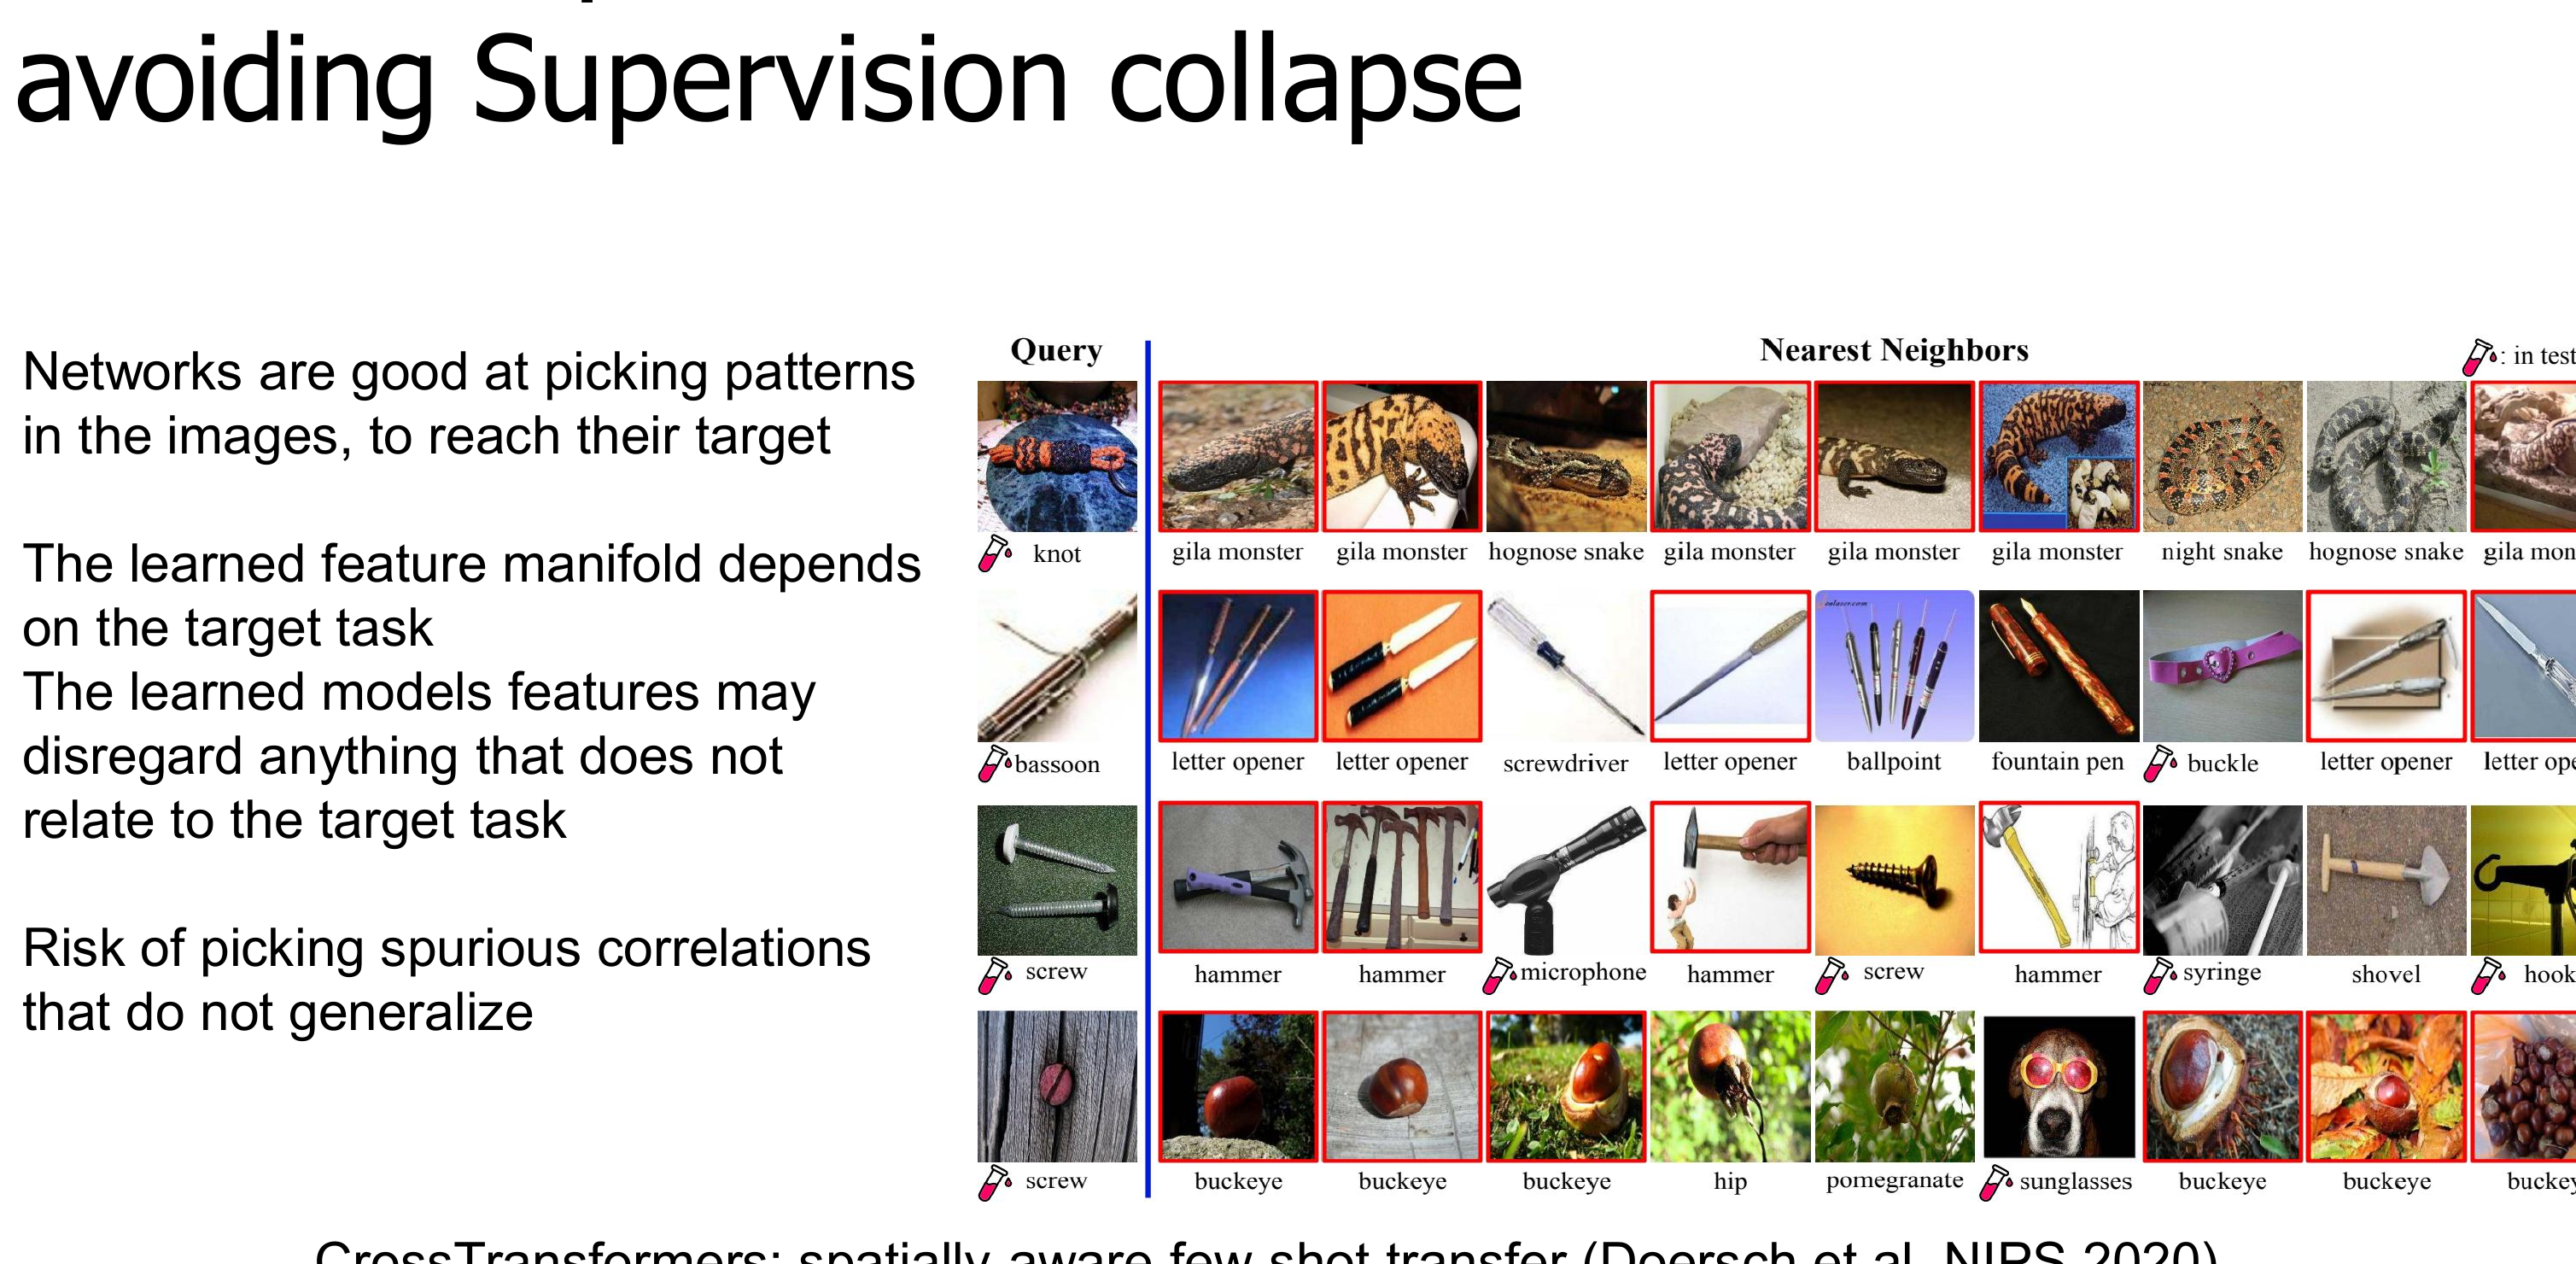
\includegraphics[width=0.90\textwidth]{Pictures/ssl_supervision_collapse_manifold.png}
    \caption{Supervision collapse in deep neural representations (from course slides~\cite{galasso2025ssl}). When trained solely on class labels, the learned manifold is constricted to features that discriminate between target classes, ignoring broader semantic structures and risking the exploitation of spurious shortcuts.}\label{fig:ssl_supervision_collapse}
\end{figure}

To resolve this fundamental tension, \textbf{Self-Supervised Learning (SSL)} re-frames representation learning: rather than relying on human annotations, the training signal is derived directly from the intrinsic structure of the unlabeled data itself. 

This chapter formalizes the principles, mathematical formulations, and evolutionary milestones of self-supervised visual representation learning, following the curriculum designed by Prof.~Fabio Galasso~\cite{galasso2025ssl}.

---

\section{Foundations of Self-Supervised Learning}

\subsection{The Pretext-Downstream Paradigm}

The canonical self-supervised learning pipeline operates across two decoupled stages, as illustrated in Figure~\ref{fig:ssl_pretext_downstream}:

\begin{enumerate}[leftmargin=*]
    \item \textbf{Pretext Task (Self-Supervised Pre-training):} The model is trained on a massive unlabeled dataset $\mathcal{D}_{\text{unlabeled}} = \{x_1, x_2, \dots, x_N\}$. An artificial supervisory objective (a \emph{pretext task}) is defined automatically from the data without human intervention. The primary goal is not the pretext task itself, but rather forcing the feature encoder $f_\theta(\cdot)$ to extract rich, generalizable visual representations.
    \item \textbf{Downstream Task (Transfer Learning):} The pre-trained encoder $f_\theta(\cdot)$ is transferred to target tasks of interest (such as ImageNet classification, object detection, or instance segmentation) using a smaller labeled dataset $\mathcal{D}_{\text{downstream}} = {\left\{ (x_i, y_i) \right\}}_{i=1}^M$.
\end{enumerate}

\begin{figure}[htbp]
    \centering
    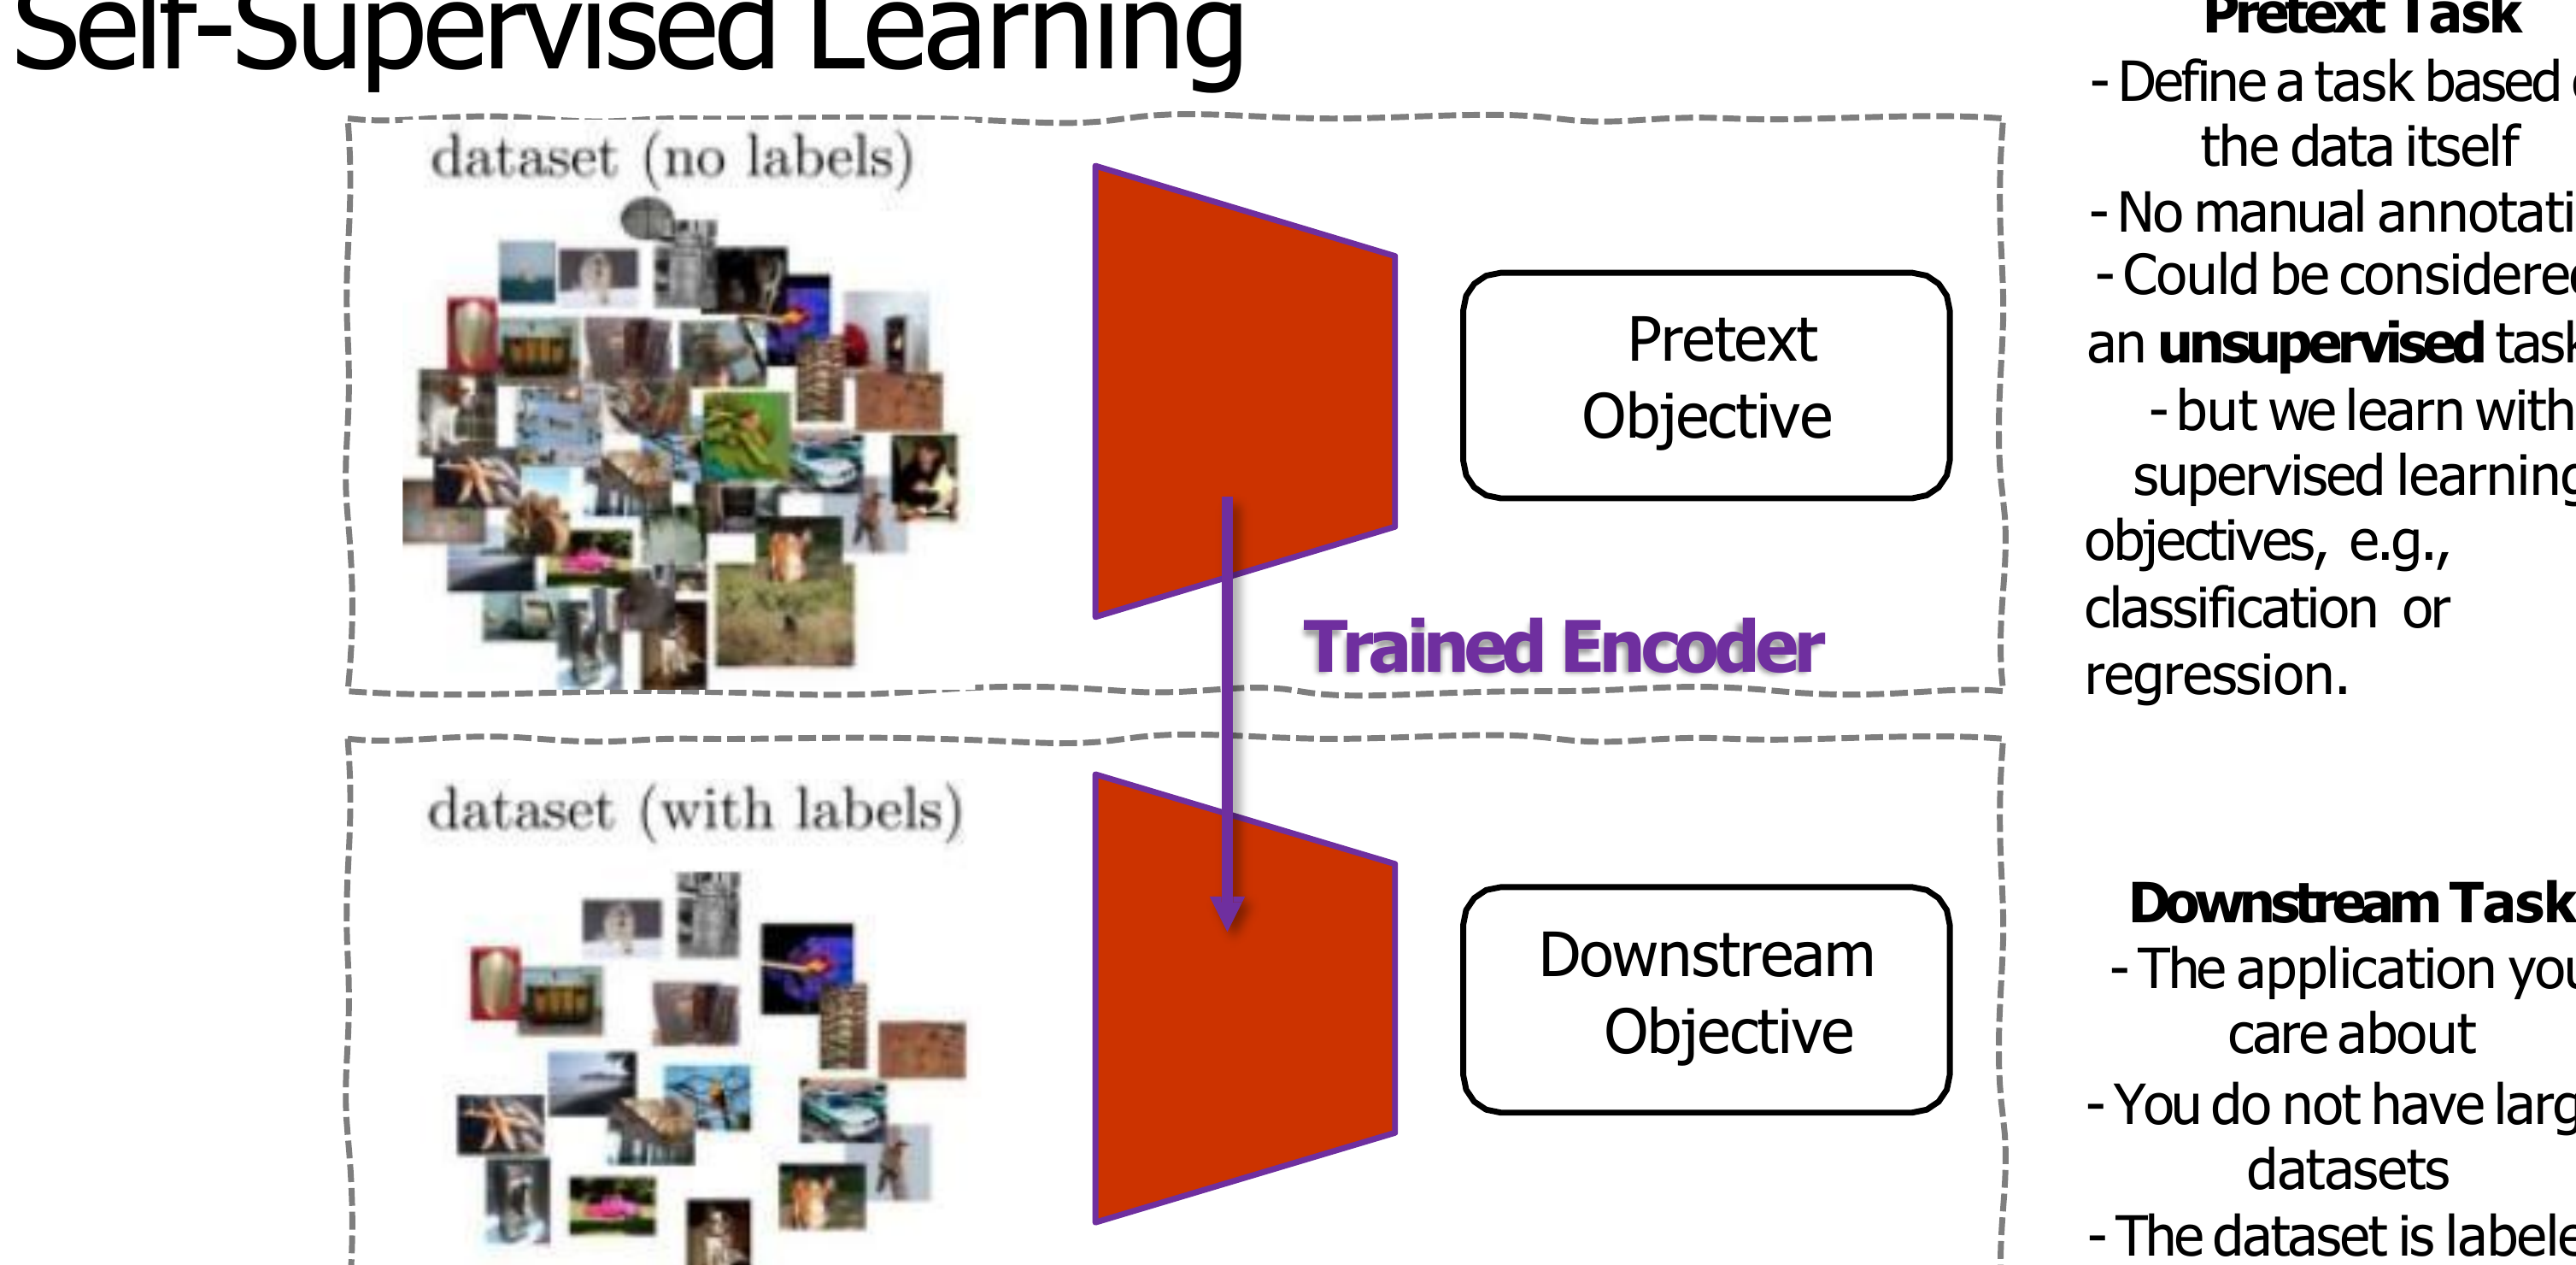
\includegraphics[width=0.90\textwidth]{Pictures/ssl_pretext_downstream_paradigm.png}
    \caption{The two-stage Self-Supervised Learning framework (from course slides~\cite{galasso2025ssl}). Left: The feature encoder $f_\theta$ is trained on an unlabeled pretext objective. Right: The learned representation is frozen or fine-tuned on target downstream tasks.}\label{fig:ssl_pretext_downstream}
\end{figure}

\subsection{Evaluation Protocols for Learned Representations}

Evaluating the quality of an unsupervised representation requires standardized empirical protocols:

\begin{enumerate}[leftmargin=*]
    \item \textbf{Pretext Task Performance:} Measuring validation accuracy or loss directly on the pretext task. While useful for monitoring convergence, pretext performance often correlates poorly with downstream utility: networks can invent clever low-level \emph{shortcuts} (such as exploiting lens chromatic aberration or edge continuity) that achieve near-perfect pretext accuracy while learning degenerate semantic representations.
    \item \textbf{Linear Evaluation Protocol (Linear Probing):} The gold standard for representation quality. The pre-trained feature extractor $f_\theta$ is completely frozen. A single linear classifier (a linear projection followed by Softmax) is trained on top of the frozen representations $h = f_\theta(x)$ on a target benchmark (e.g., ImageNet-1K):
    \begin{equation}
        \hat{y} = \text{Softmax}(W^\top f_\theta(x) + b)
    \end{equation}
    Because the backbone weights $\theta$ cannot adapt, high linear probing accuracy proves that the pre-trained features are \textbf{linearly separable} and encode rich semantic concepts natively.
    \item \textbf{Fine-Tuning Protocol:} The entire network (backbone $f_\theta$ plus a newly initialized task head) is fine-tuned end-to-end on the downstream dataset, typically using a smaller learning rate for the backbone layers. This measures the efficacy of the representation as a weight initialization strategy.
    \item \textbf{Semi-Supervised Benchmark:} The pre-trained model is fine-tuned on extreme low-data regimes, such as $1\%$ or $10\%$ of labeled ImageNet examples. Superior representations yield competitive performance even when labels are drastically scarce.
\end{enumerate}

---

\section{Heuristic Pretext Tasks}

Early self-supervised methods relied on clever, domain-specific heuristic transformations where the input image is perturbed and the network is tasked with predicting the perturbation parameters.

\subsection{Predicting Geometric Rotations}

Gidaris et al.~\cite{gidaris2018unsupervised} proposed training a convolutional network to predict discrete geometric rotations applied to an image. Given an unrotated, upright image $x$, a transformation operator $R_y(x)$ rotates the image by $y \in \{0^\circ, 90^\circ, 180^\circ, 270^\circ\}$ (represented as a 4-class categorical label $y \in \{0, 1, 2, 3\}$), as depicted in Figure~\ref{fig:ssl_rotation_prediction}:
\begin{equation}
    \mathcal{L}_{\text{rot}} = - \sum_{k=0}^3 \mathbb{I}_{[y = k]} \log \left( \frac{\exp(w_k^\top f_\theta(R_y(x)))}{\sum_{j=0}^3 \exp(w_j^\top f_\theta(R_y(x)))} \right)
\end{equation}

\begin{figure}[htbp]
    \centering
    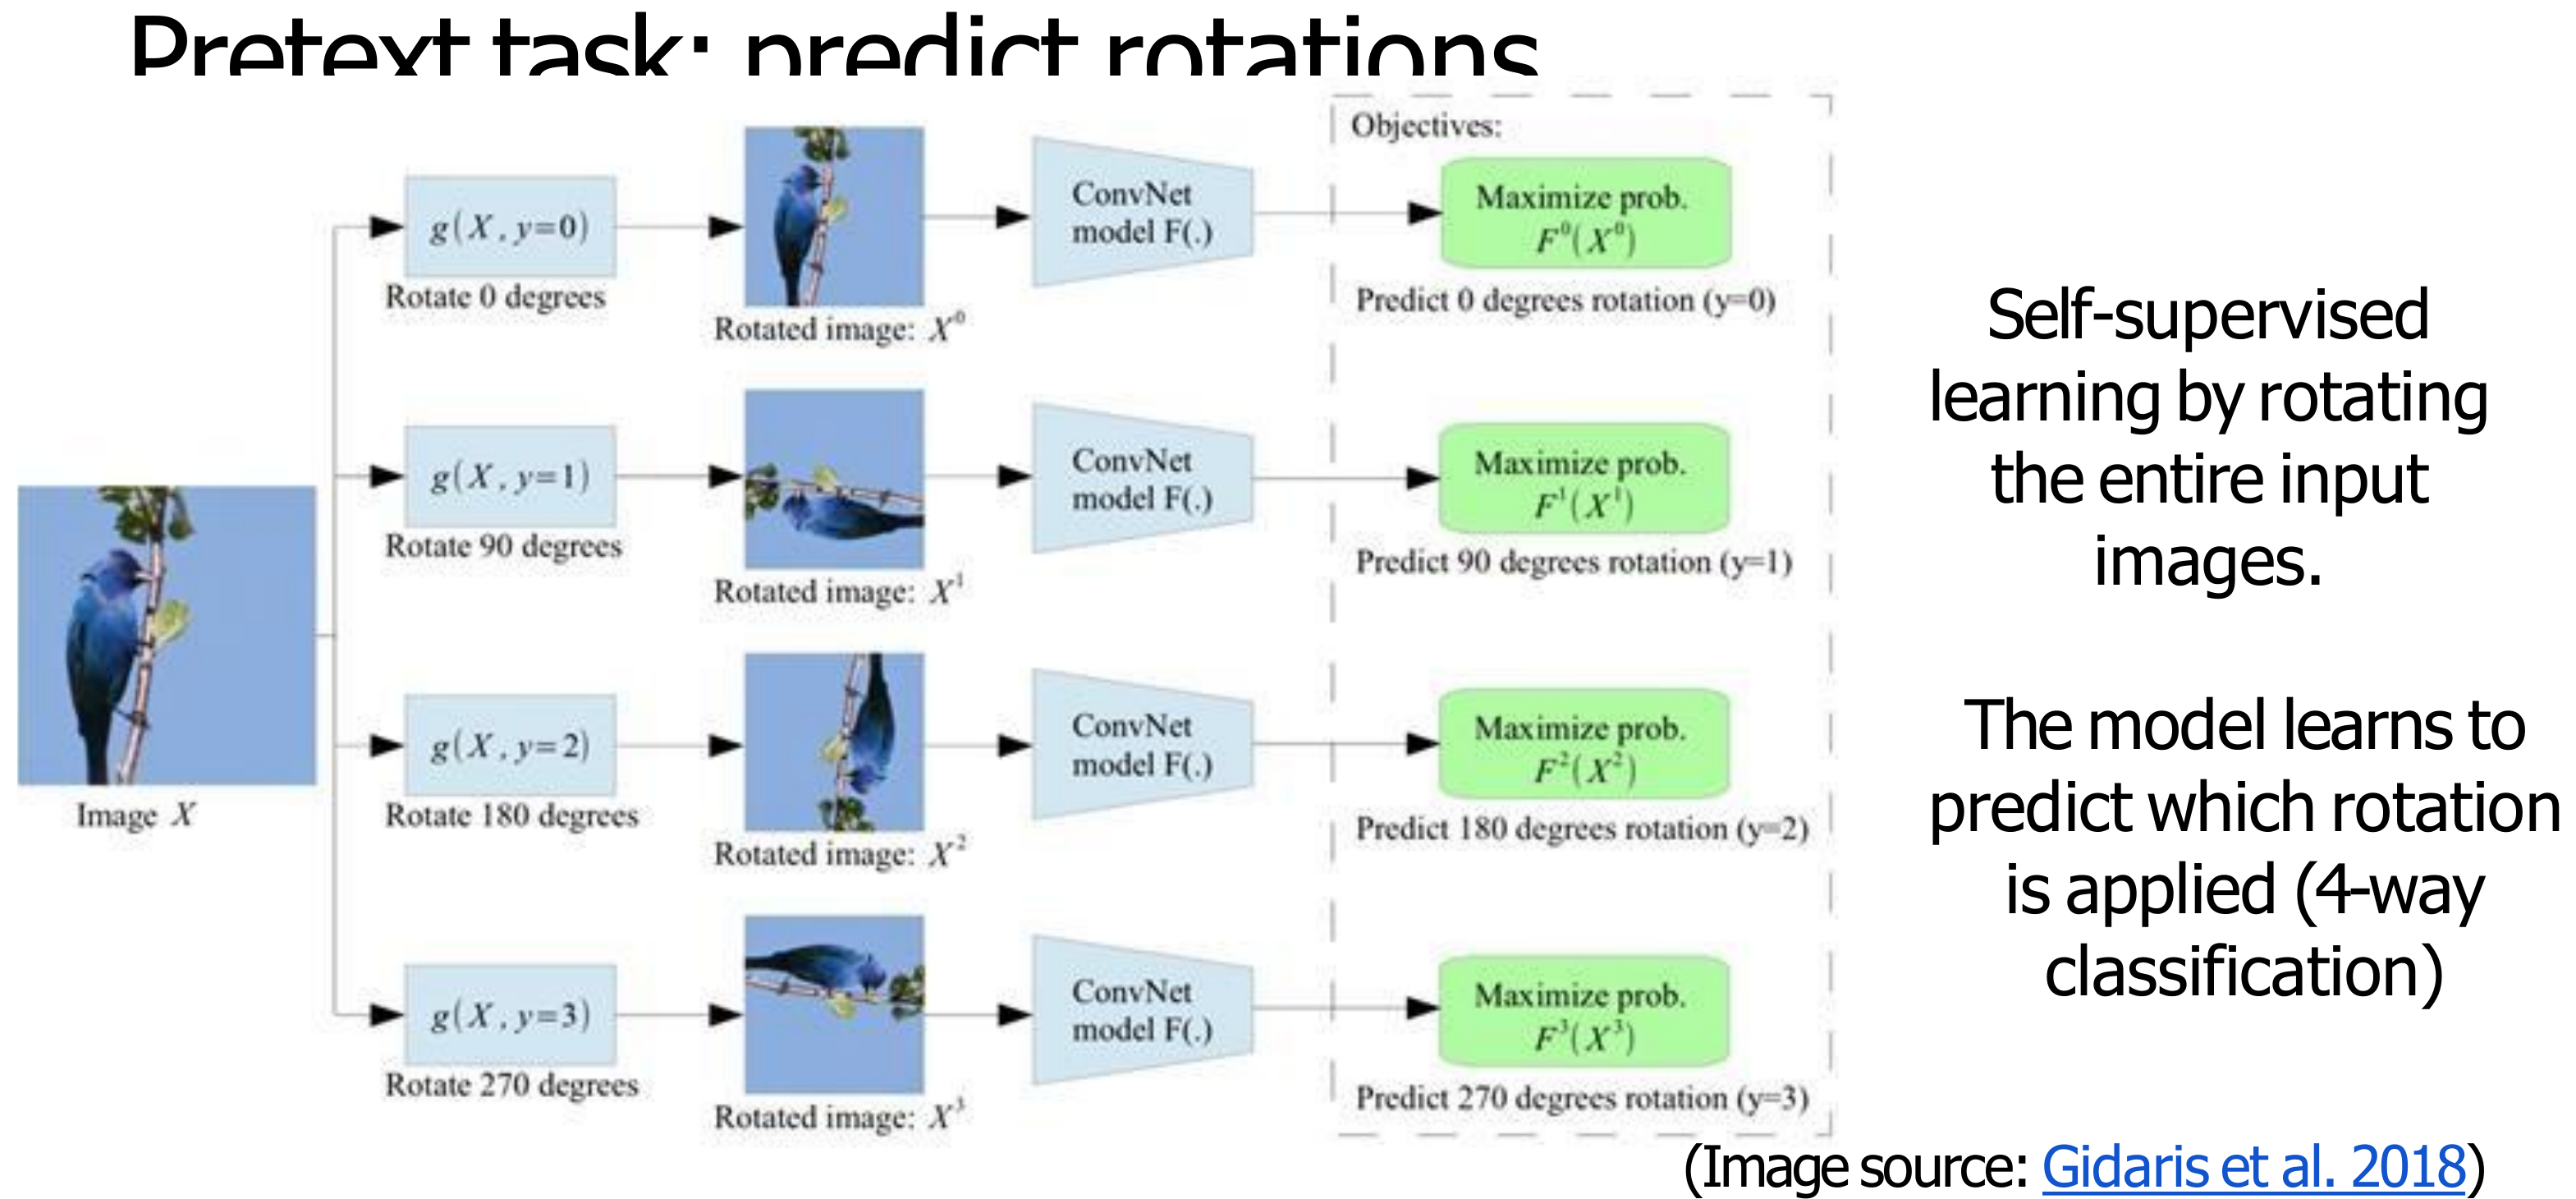
\includegraphics[width=0.90\textwidth]{Pictures/ssl_rotation_prediction.png}
    \caption{Rotation prediction pretext task (from course slides~\cite{galasso2025ssl, gidaris2018unsupervised}). The network receives an image rotated by $0^\circ$, $90^\circ$, $180^\circ$, or $270^\circ$ and must classify the applied angle.}\label{fig:ssl_rotation_prediction}
\end{figure}

\begin{InsightBox}
\textbf{Why Rotation Prediction Induces Semantic Understanding:} \\
A model cannot recognize whether a dog or a building is upside-down ($180^\circ$) by inspecting isolated, low-level pixel statistics alone. To determine canonical orientation, the network must identify high-level visual entities, localize object parts (e.g., eyes, wheels, sky, ground), and reason about physical gravity.
\end{InsightBox}

\subsection{Spatial Context: Relative Patch Location and Jigsaw Puzzles}

\subsubsection{Relative Patch Localization}
Doersch et al.~\cite{doersch2015unsupervised} formulated an unsupervised spatial context task. As shown in Figure~\ref{fig:ssl_patch_relative_location}, two random patches are extracted from a $3 \times 3$ grid: a central patch and one of eight peripheral neighbors. The network must predict the relative spatial position $y \in \{1, \dots, 8\}$.

\begin{figure}[htbp]
    \centering
    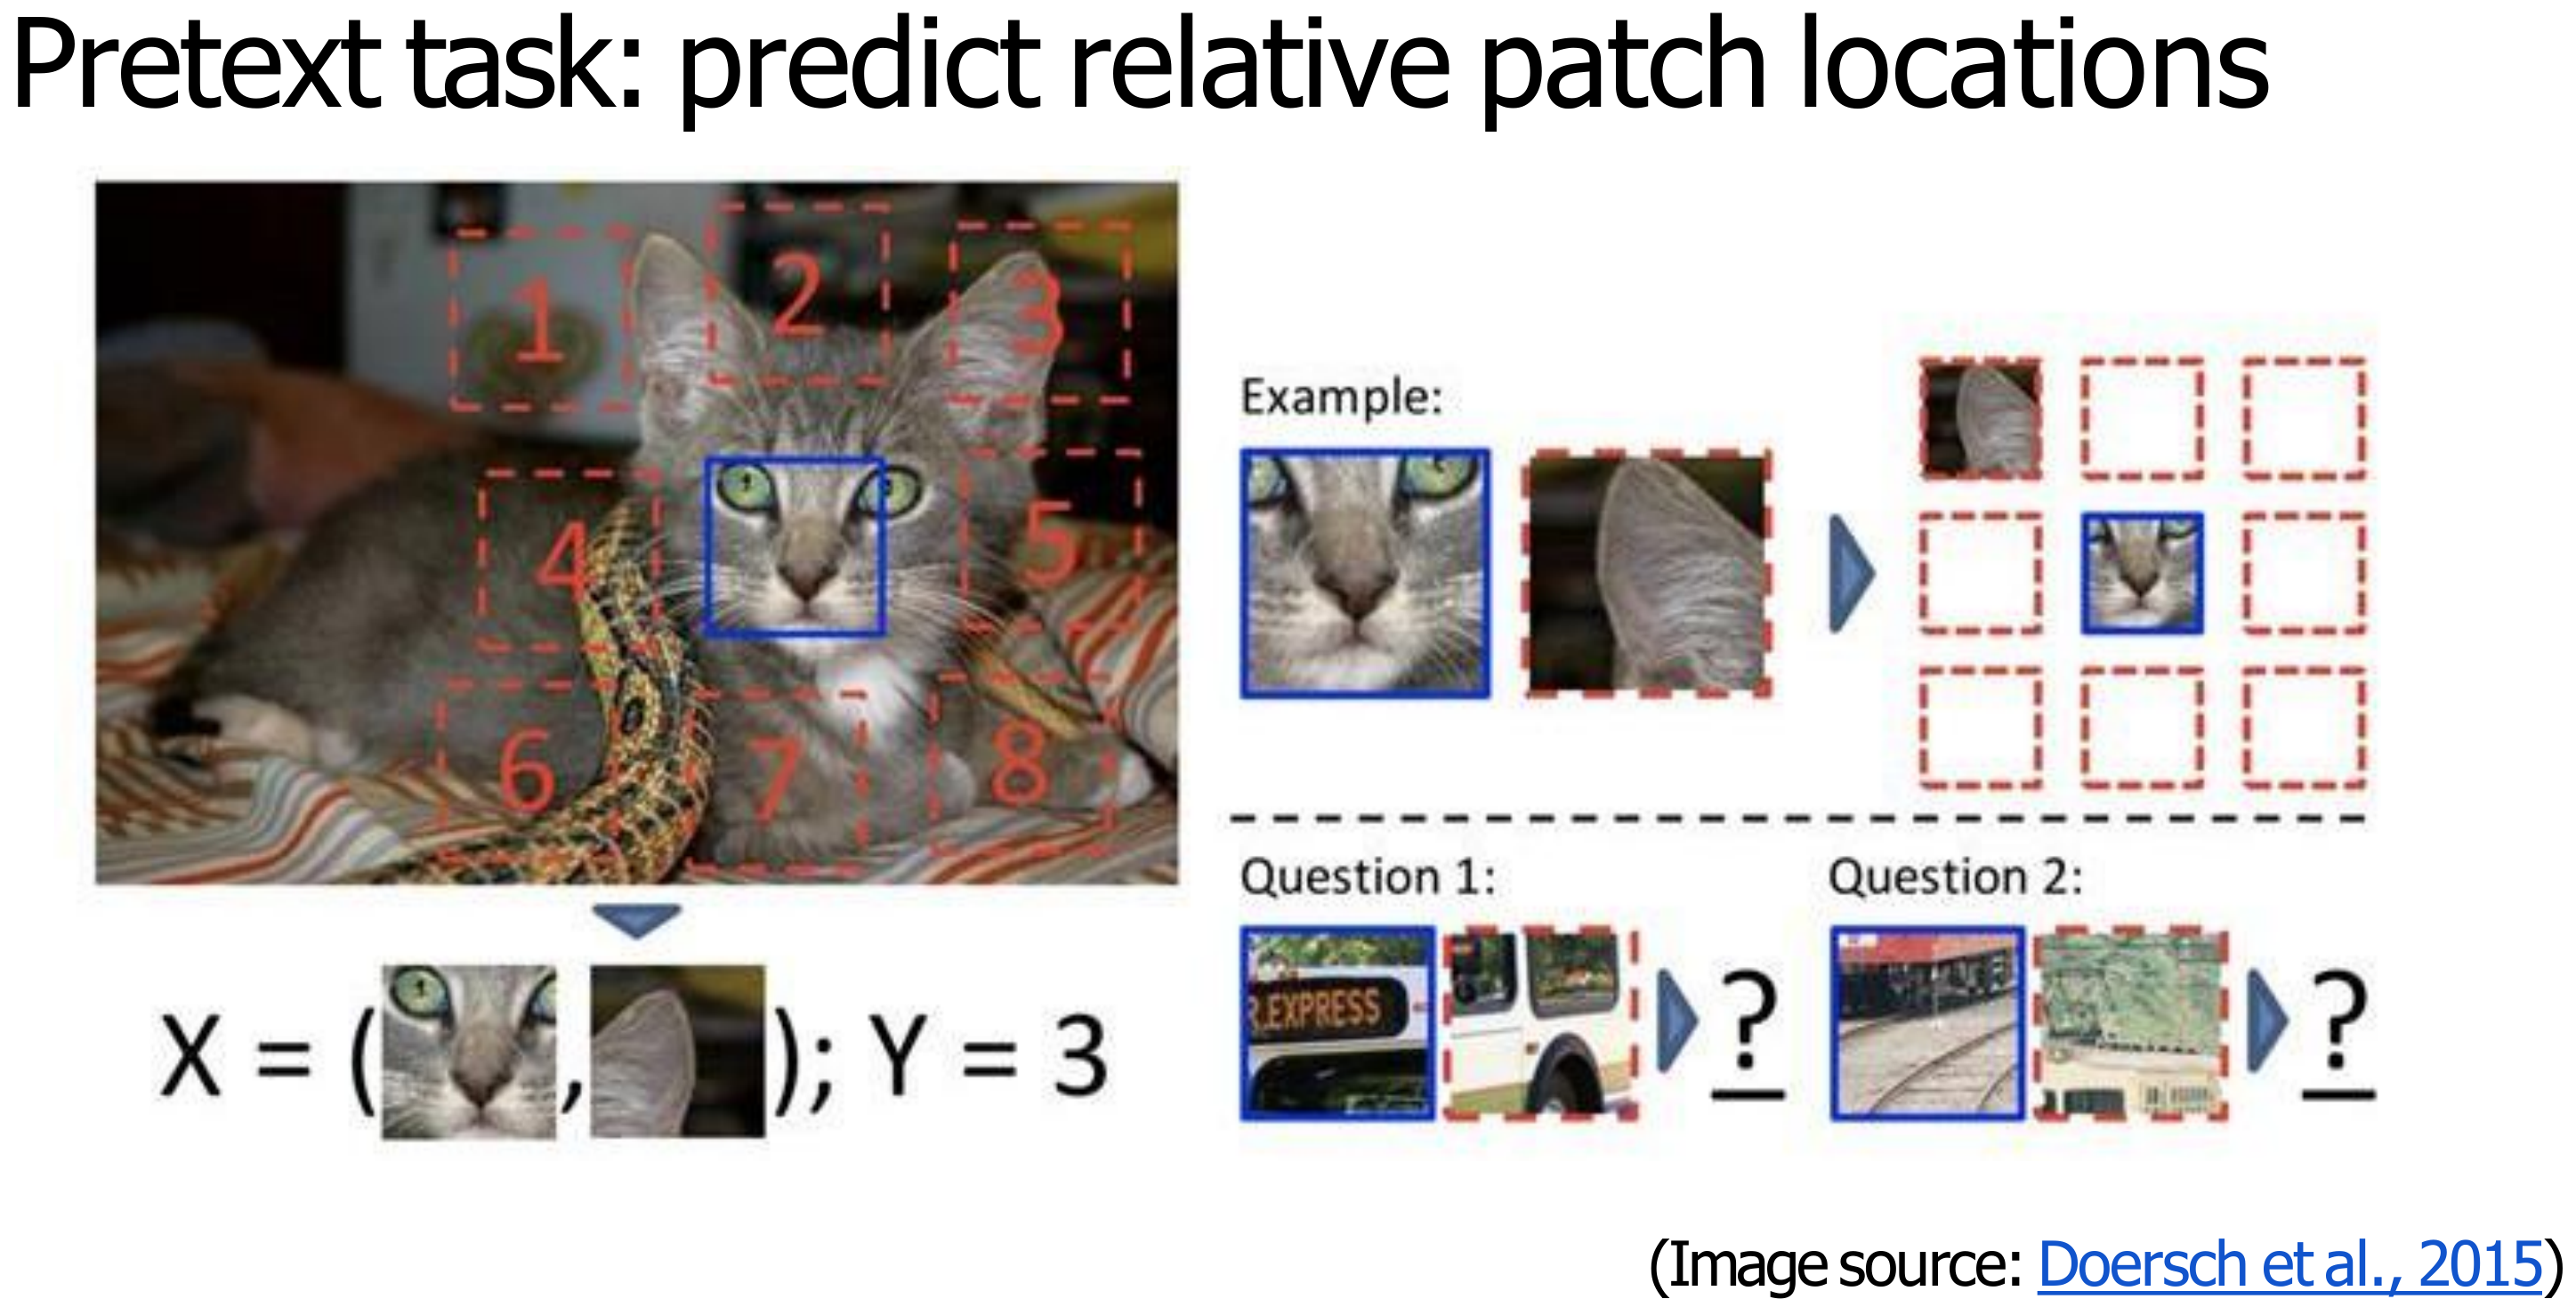
\includegraphics[width=0.88\textwidth]{Pictures/ssl_patch_relative_location.png}
    \caption{Relative patch location pretext task (from course slides~\cite{galasso2025ssl, doersch2015unsupervised}). The network takes two patches (one central, one random neighbor) and predicts which of the eight spatial positions the neighbor occupies.}\label{fig:ssl_patch_relative_location}
\end{figure}

To prevent the model from exploiting trivial shortcuts, two key design safeguards are mandatory:
\begin{itemize}[leftmargin=*]
    \item \textbf{Random Gap and Jitter:} If patches were strictly adjacent, the network could trivially align continuous edge contours across patch boundaries. Random spatial gaps between patches eliminate edge continuity shortcuts.
    \item \textbf{Color Jittering and Aberration Removal:} Optical camera lenses exhibit \emph{chromatic aberration}---a radial distortion where color channels separate slightly toward image borders. Networks quickly learn to evaluate the radial color shift to deduce absolute patch position! Converting patches to grayscale or randomly dropping color channels eliminates this hardware shortcut.
\end{itemize}

\subsubsection{Solving Jigsaw Puzzles}
Noroozi and Favaro~\cite{noroozi2016unsupervised} extended spatial context prediction to an entire $3 \times 3$ grid of 9 patches, shown in Figure~\ref{fig:ssl_jigsaw_puzzle}. Rather than predicting single pair relations, the 9 patches are permuted according to a pre-defined permutation set $\mathcal{P} \subset S_9$ (typically $|\mathcal{P}| = 100$ or $1000$ permutations chosen with maximum Hamming distance out of $9! = 362{,}880$ possibilities). 

\begin{figure}[htbp]
    \centering
    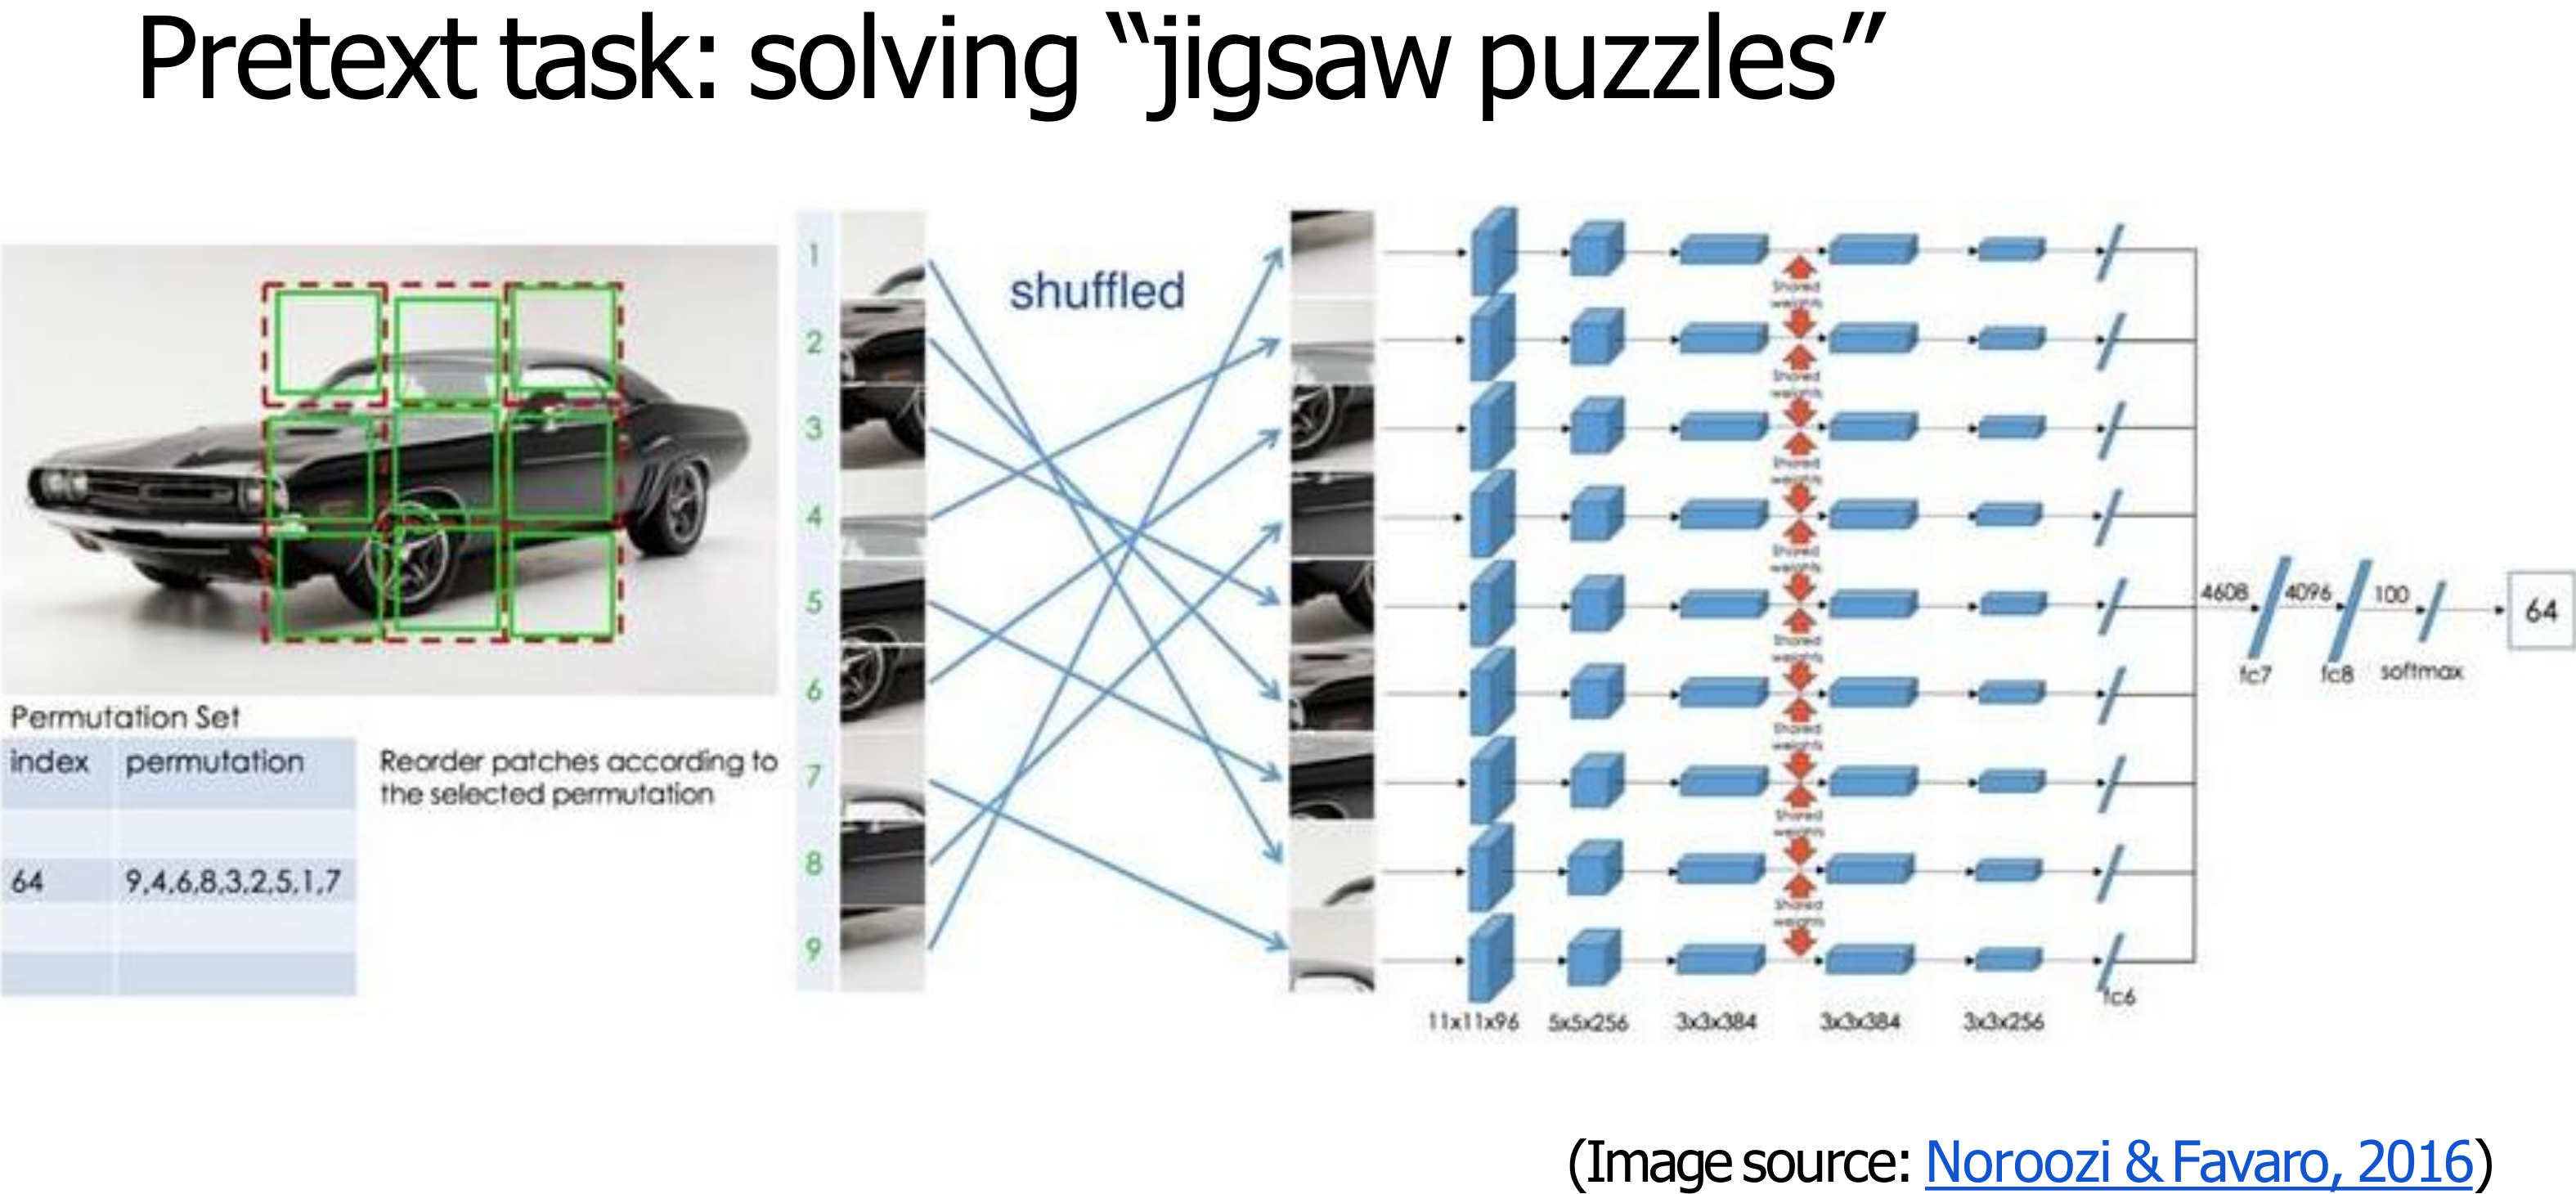
\includegraphics[width=0.92\textwidth]{Pictures/ssl_jigsaw_puzzle_cfn.png}
    \caption{Solving Jigsaw Puzzles with Context-Free Networks (CFN) (from course slides~\cite{galasso2025ssl, noroozi2016unsupervised}). 9 randomly shuffled patches pass through weight-shared convolutional towers before a fully connected classifier predicts the permutation index.}\label{fig:ssl_jigsaw_puzzle}
\end{figure}

The architecture, termed a \textbf{Context-Free Network (CFN)}, processes each patch independently through weight-shared Siamese convolutional backbones before concatenating the features into an MLP classifier. This ensures the convolutional kernels extract modular, position-agnostic part representations.

\subsection{Context Encoders: Feature Learning by Inpainting}

Pathak et al.~\cite{pathak2016context} introduced \textbf{Context Encoders}, where an encoder-decoder network reconstructs a missing central image region (e.g., a $64 \times 64$ masked region within a $128 \times 128$ image), as illustrated in Figure~\ref{fig:ssl_context_encoders}.

\begin{figure}[htbp]
    \centering
    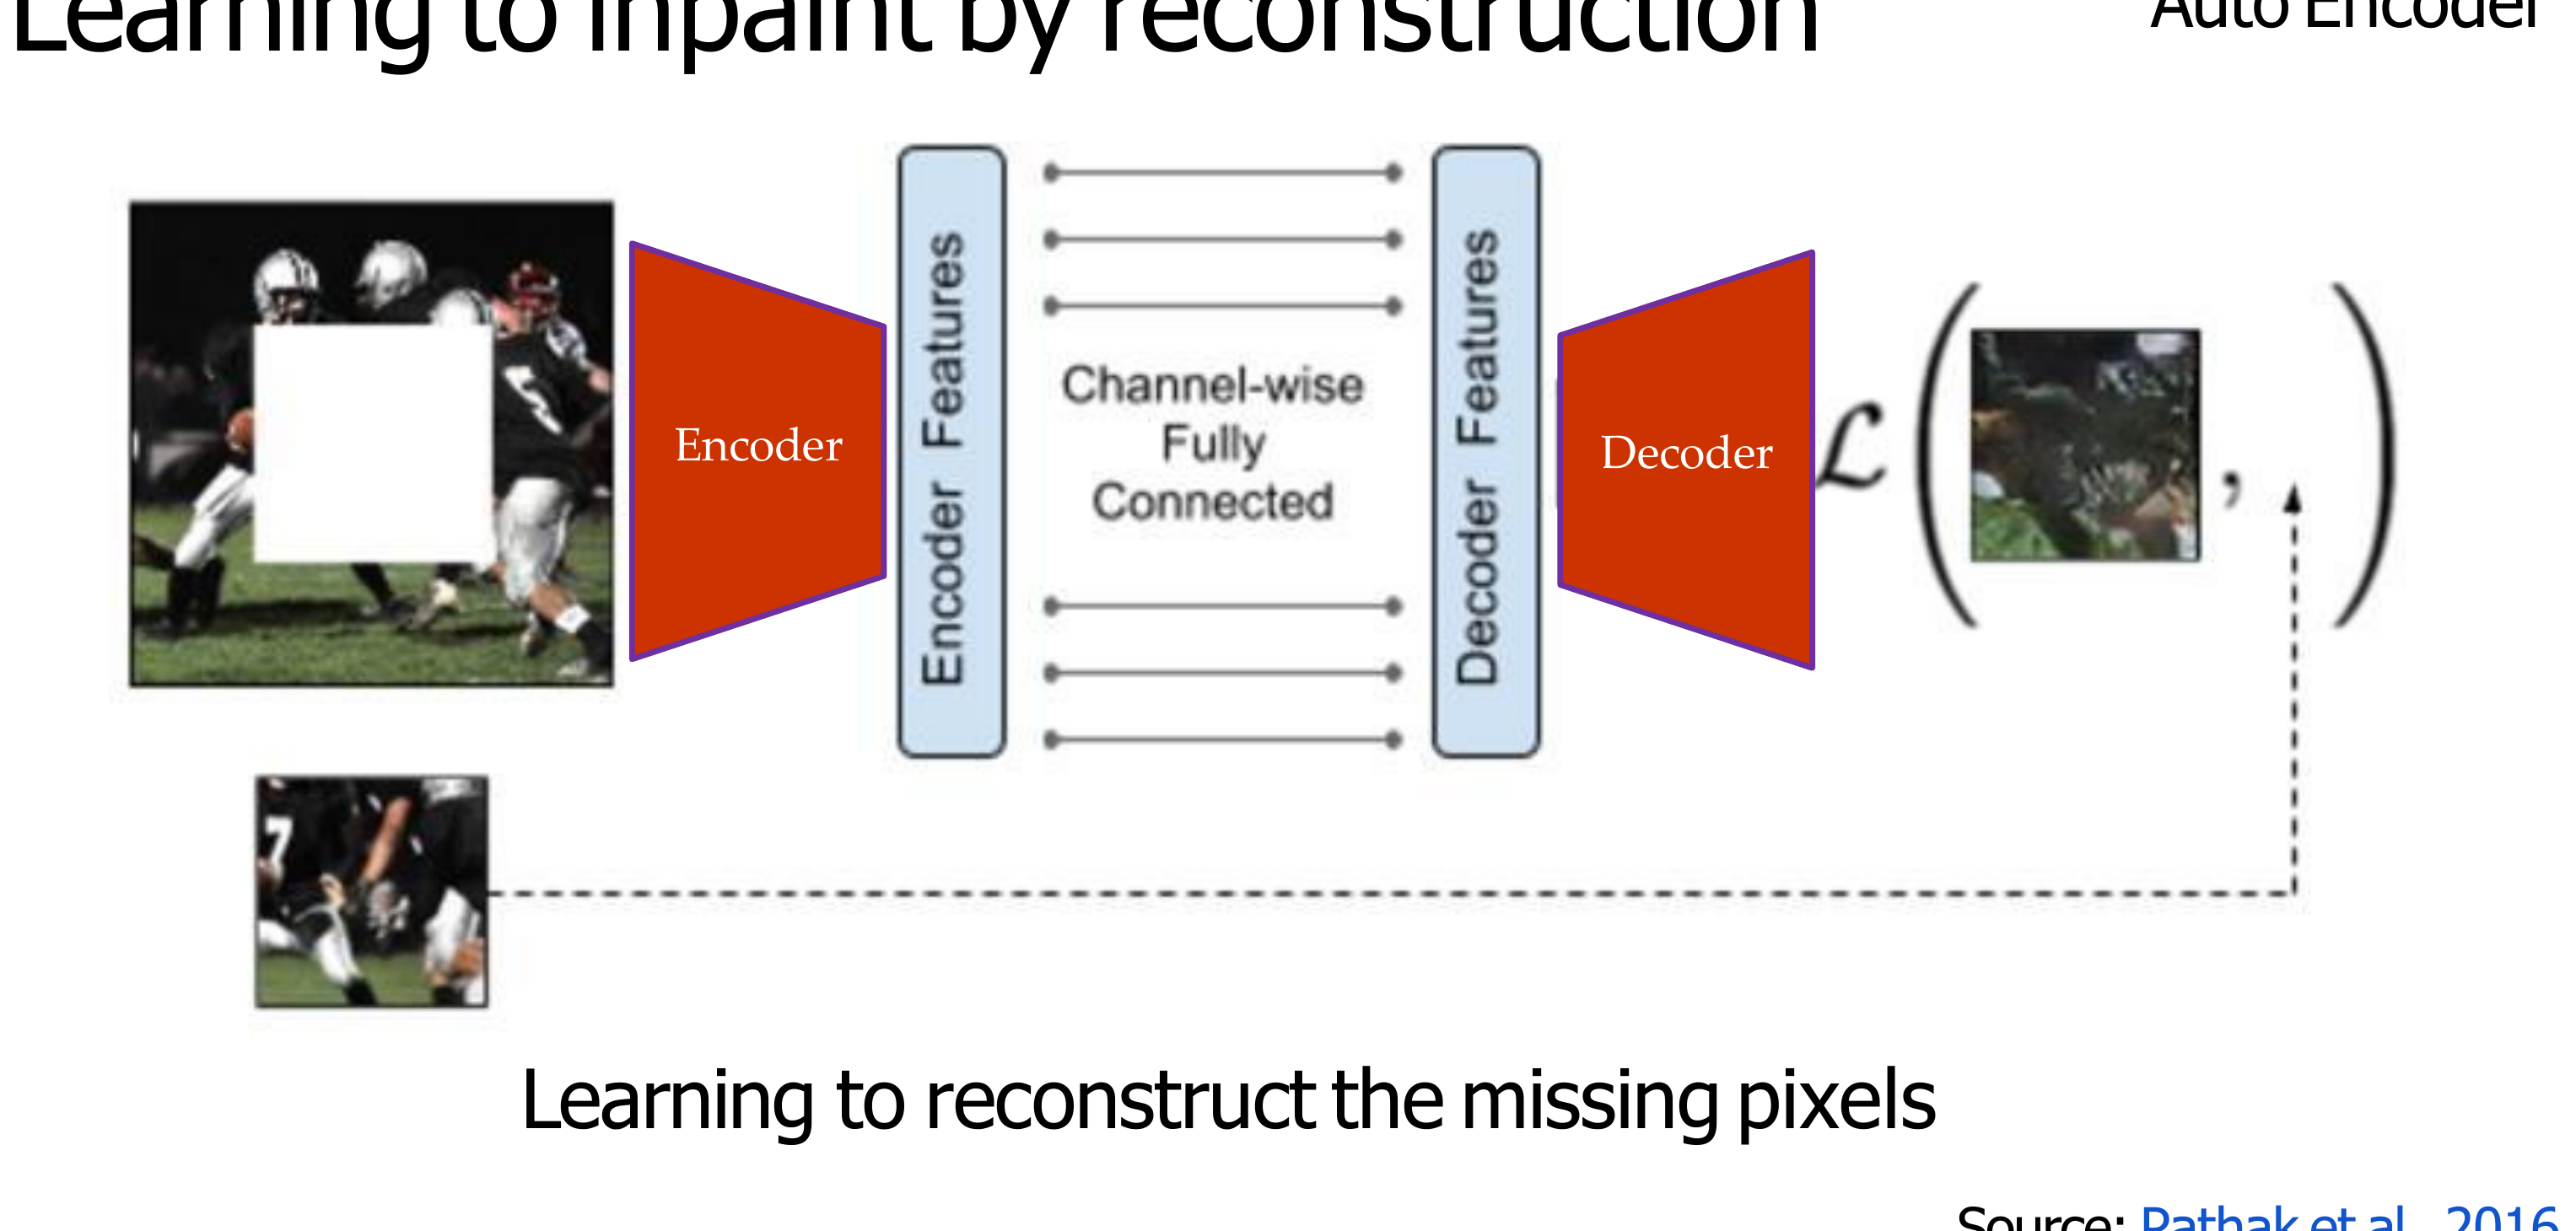
\includegraphics[width=0.90\textwidth]{Pictures/ssl_context_encoders_inpainting.png}
    \caption{Context Encoders for image inpainting (from course slides~\cite{galasso2025ssl, pathak2016context}). An encoder compresses the unmasked context into a latent representation, and a decoder reconstructs the missing pixel patch via a joint reconstruction and adversarial loss.}\label{fig:ssl_context_encoders}
\end{figure}

Training with standard $L_2$ pixel reconstruction loss alone:
\begin{equation}
    \mathcal{L}_{\text{recon}} = \|\hat{M} \odot (x - f_\theta((1 - \hat{M}) \odot x))\|_2^2
\end{equation}
penalizes variance and forces the network to output the blurry expected average of all plausible completions. To generate sharp, semantically realistic structures, Pathak et al.\@ combined the reconstruction loss with a Generative Adversarial Network (GAN) adversarial objective:
\begin{equation}
    \mathcal{L}_{\text{total}} = \mathcal{L}_{\text{recon}} + \lambda_{\text{adv}} \mathcal{L}_{\text{adv}}
\end{equation}
where an auxiliary discriminator $D_\phi$ distinguishes real unmasked image patches from synthesized completions.

\subsection{Image and Video Colorization}

\subsubsection{Colorful Image Colorization and Split-Brain Autoencoders}
Zhang et al.~\cite{zhang2016colorful} formulated colorization as a pretext task: given the grayscale luminance channel $L \in \mathbb{R}^{H \times W \times 1}$ in the CIELAB color space, predict the associated color channels $ab \in \mathbb{R}^{H \times W \times 2}$. Because regression directly to continuous $a, b$ values causes desaturated, brownish predictions, Zhang et al.\@ quantized the $ab$ space into 313 discrete bins and applied class rebalancing to overweight rare, vibrant colors.

Zhang et al.~\cite{zhang2017split} subsequently generalized this into \textbf{Split-Brain Autoencoders}, shown in Figure~\ref{fig:ssl_split_brain}. Rather than reconstructing identical inputs, the input channels are split into disjoint subsets $X_1$ (e.g., $L$) and $X_2$ (e.g., $ab$). Subnetwork $f_1$ predicts $X_2$ from $X_1$, while subnetwork $f_2$ predicts $X_1$ from $X_2$:
\begin{equation}
    \mathcal{L}_{\text{split}} = \mathcal{L}(f_1(X_1), X_2) + \mathcal{L}(f_2(X_2), X_1)
\end{equation}
By forcing cross-channel prediction, the network cannot learn identity shortcuts and must construct dense, cross-modal semantic feature spaces.

\begin{figure}[htbp]
    \centering
    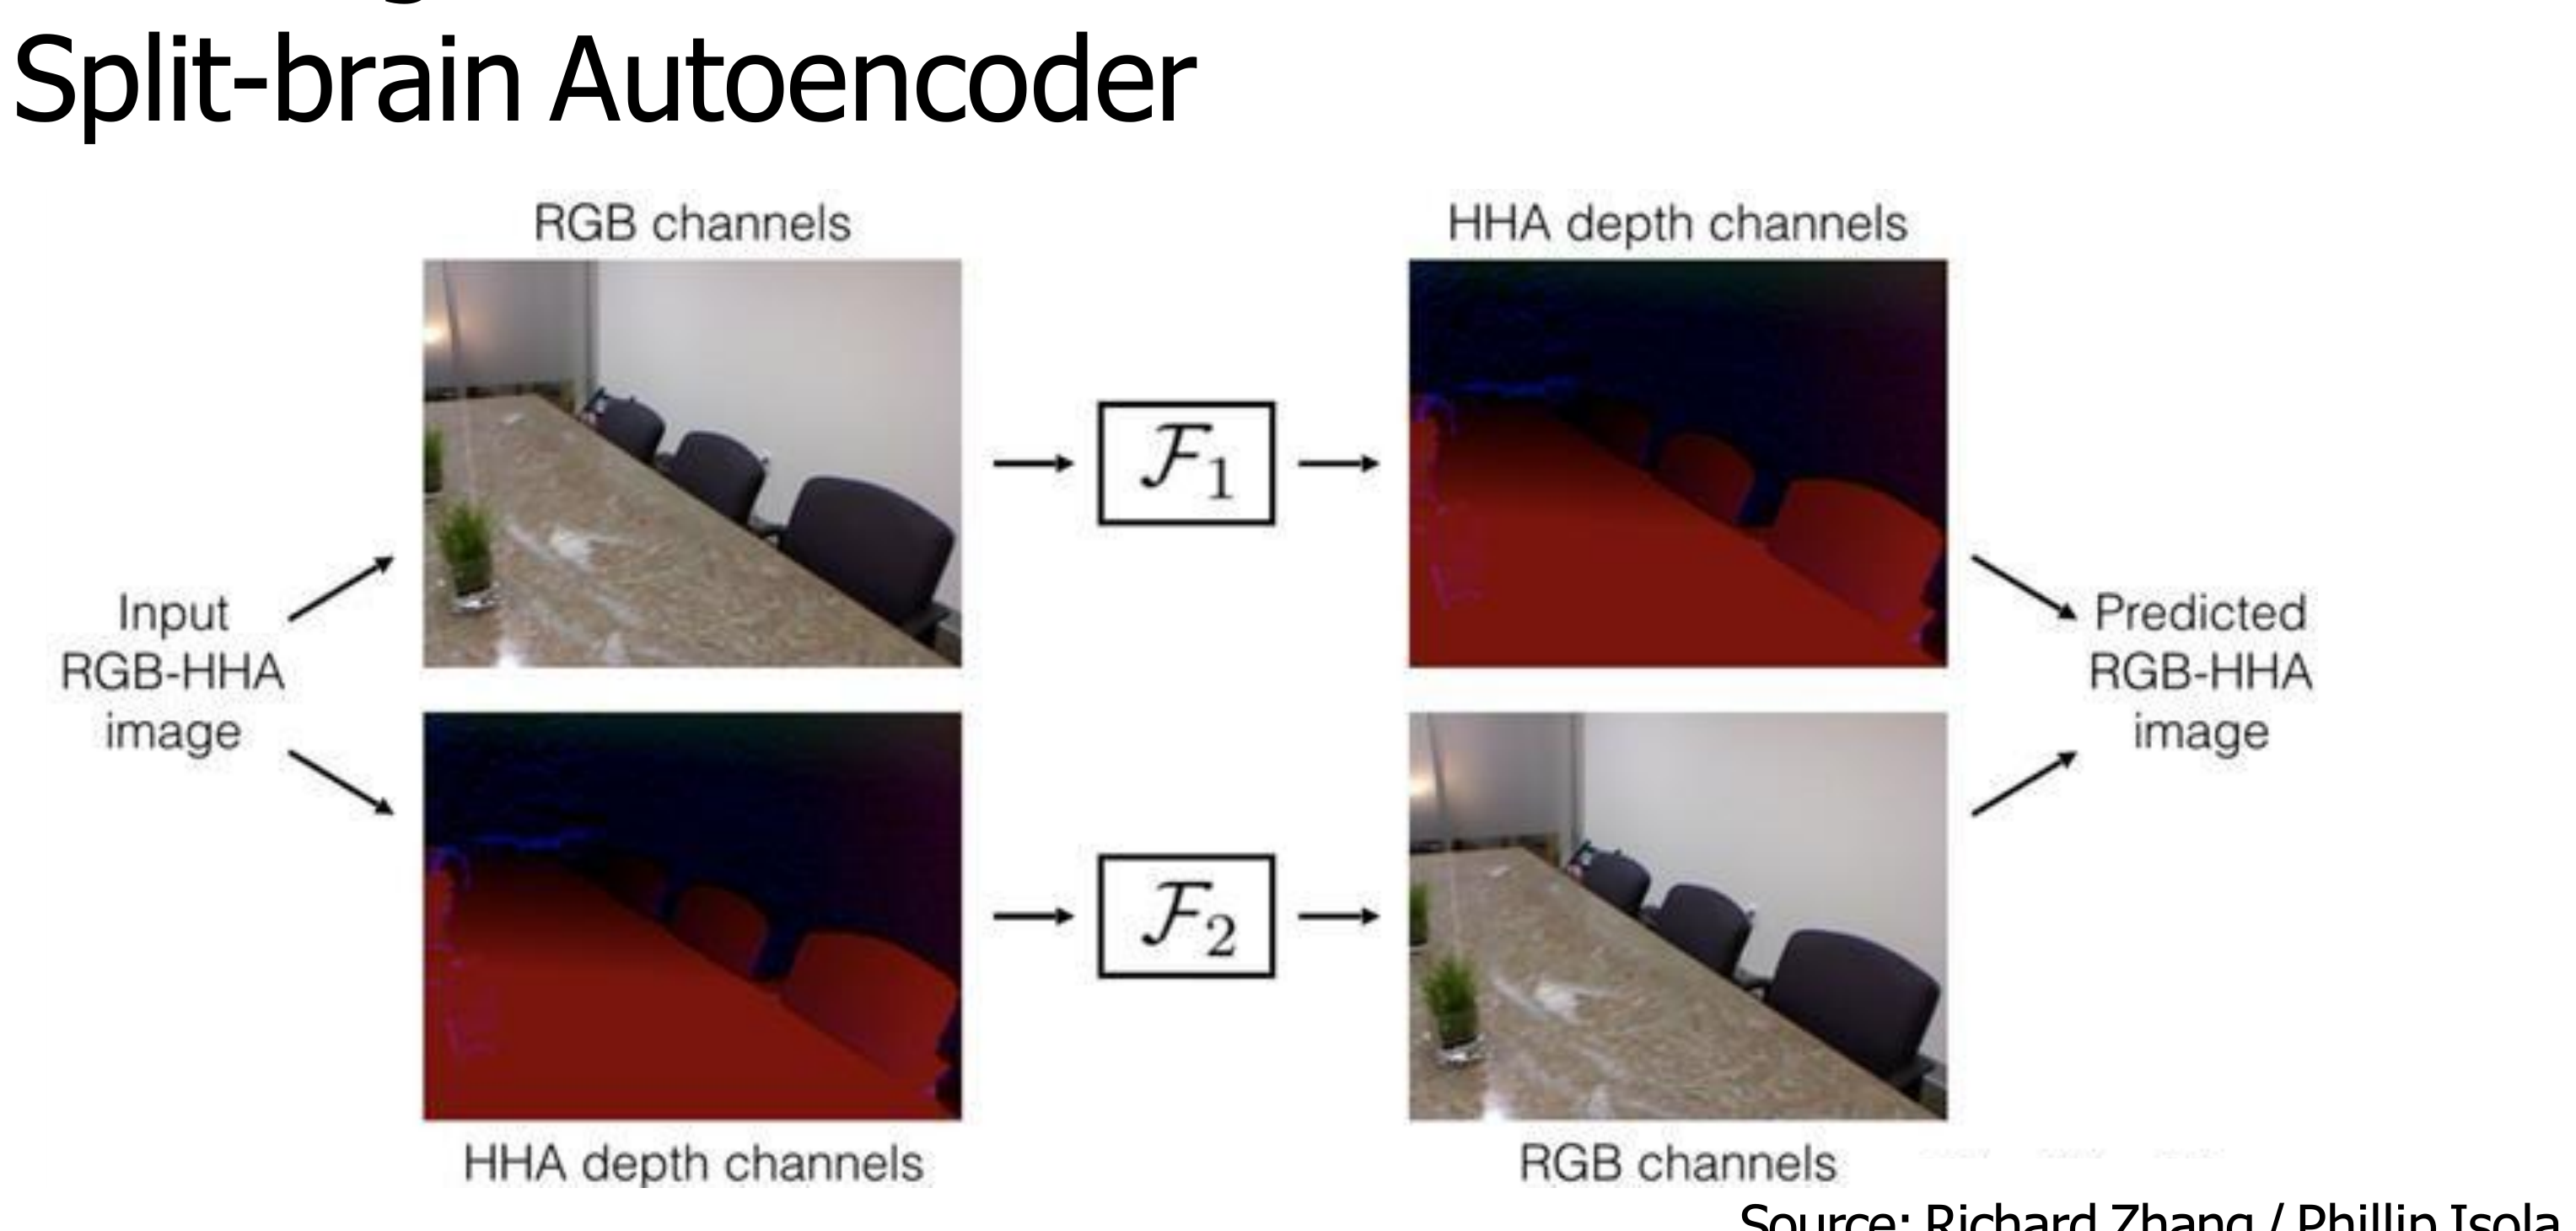
\includegraphics[width=0.88\textwidth]{Pictures/ssl_split_brain_colorization.png}
    \caption{Split-Brain Autoencoder architecture (from course slides~\cite{galasso2025ssl, zhang2017split}). Channels are partitioned into complementary subsets, forcing subnetworks to predict missing channels from observed channels without shortcutting.}\label{fig:ssl_split_brain}
\end{figure}

\subsubsection{Video Colorization and Emergence of Space-Time Tracking}
Vondrick et al.~\cite{vondrick2018tracking} leveraged temporal coherence in unlabeled video sequences. In continuous video, objects maintain consistent color over time. Given a reference frame with known color and subsequent target frames in grayscale, the network must colorize the target frames by attending to the reference frame.

\begin{figure}[htbp]
    \centering
    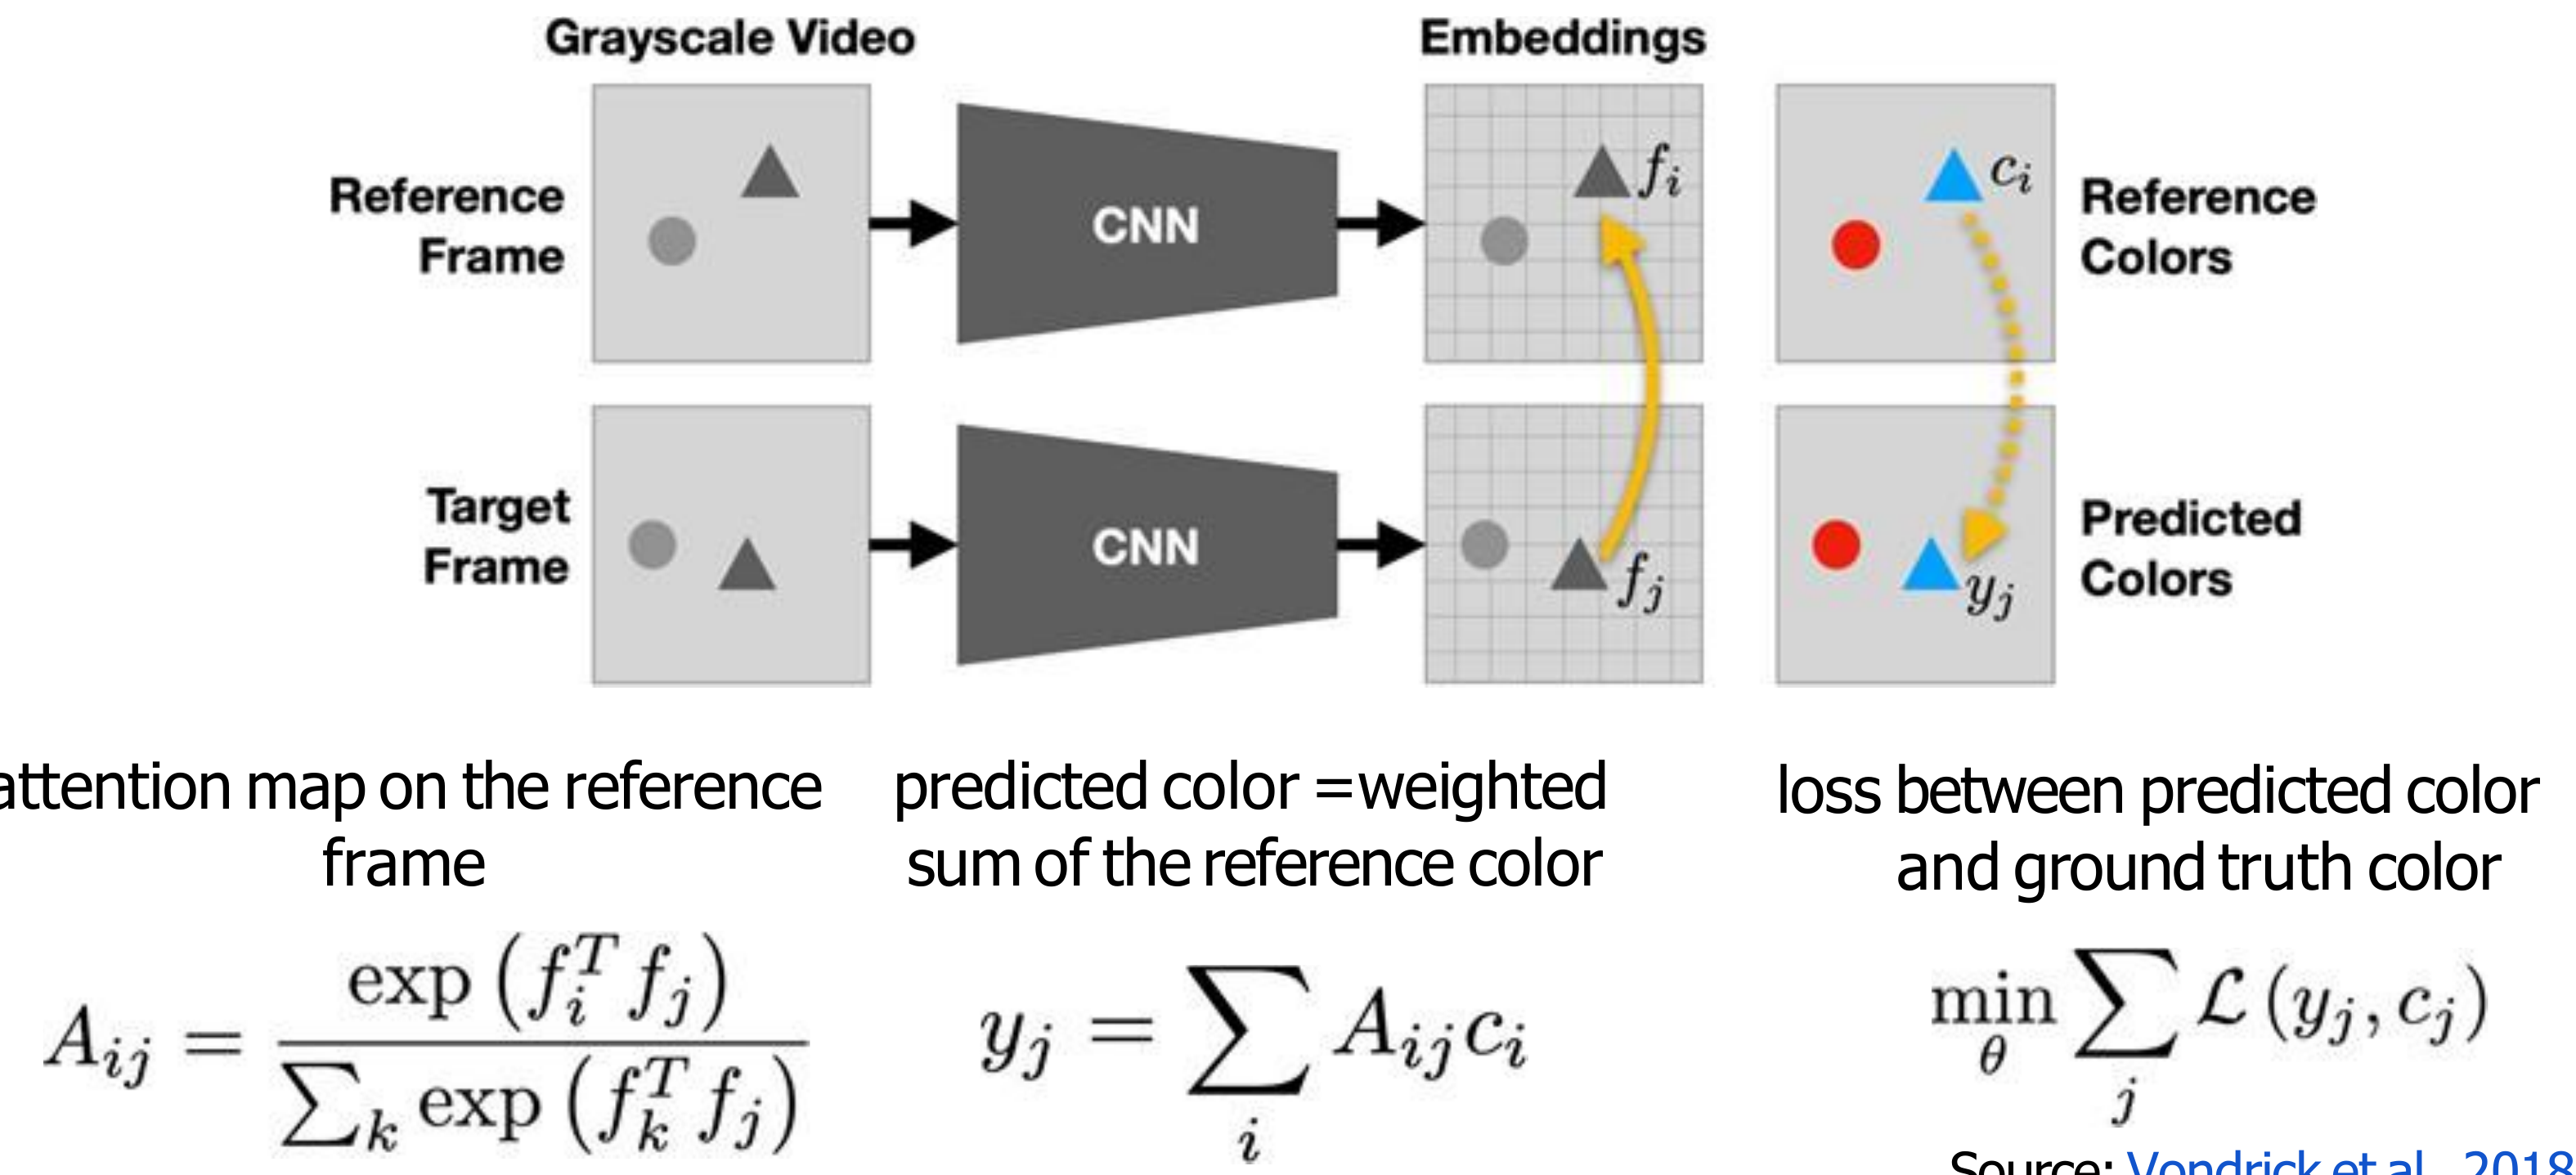
\includegraphics[width=0.90\textwidth]{Pictures/ssl_video_colorization_attention.png}
    \caption{Video colorization via space-time correspondence attention (from course slides~\cite{galasso2025ssl, vondrick2018tracking}). The network calculates dense similarity between target grayscale patches and reference colored patches.}\label{fig:ssl_video_colorization}
\end{figure}

The model maps reference patches $j$ to embeddings $g_j$ and target patches $i$ to embeddings $f_i$. A Softmax attention map $A_{ij}$ evaluates spatial-temporal similarity:
\begin{equation}
    A_{ij} = \frac{\exp(f_i^\top g_j)}{\sum_k \exp(f_i^\top g_k)}
\end{equation}
The predicted target color is computed as a weighted combination of reference colors: $\hat{c}_i = \sum_j A_{ij} c_j$.

\begin{figure}[htbp]
    \centering
    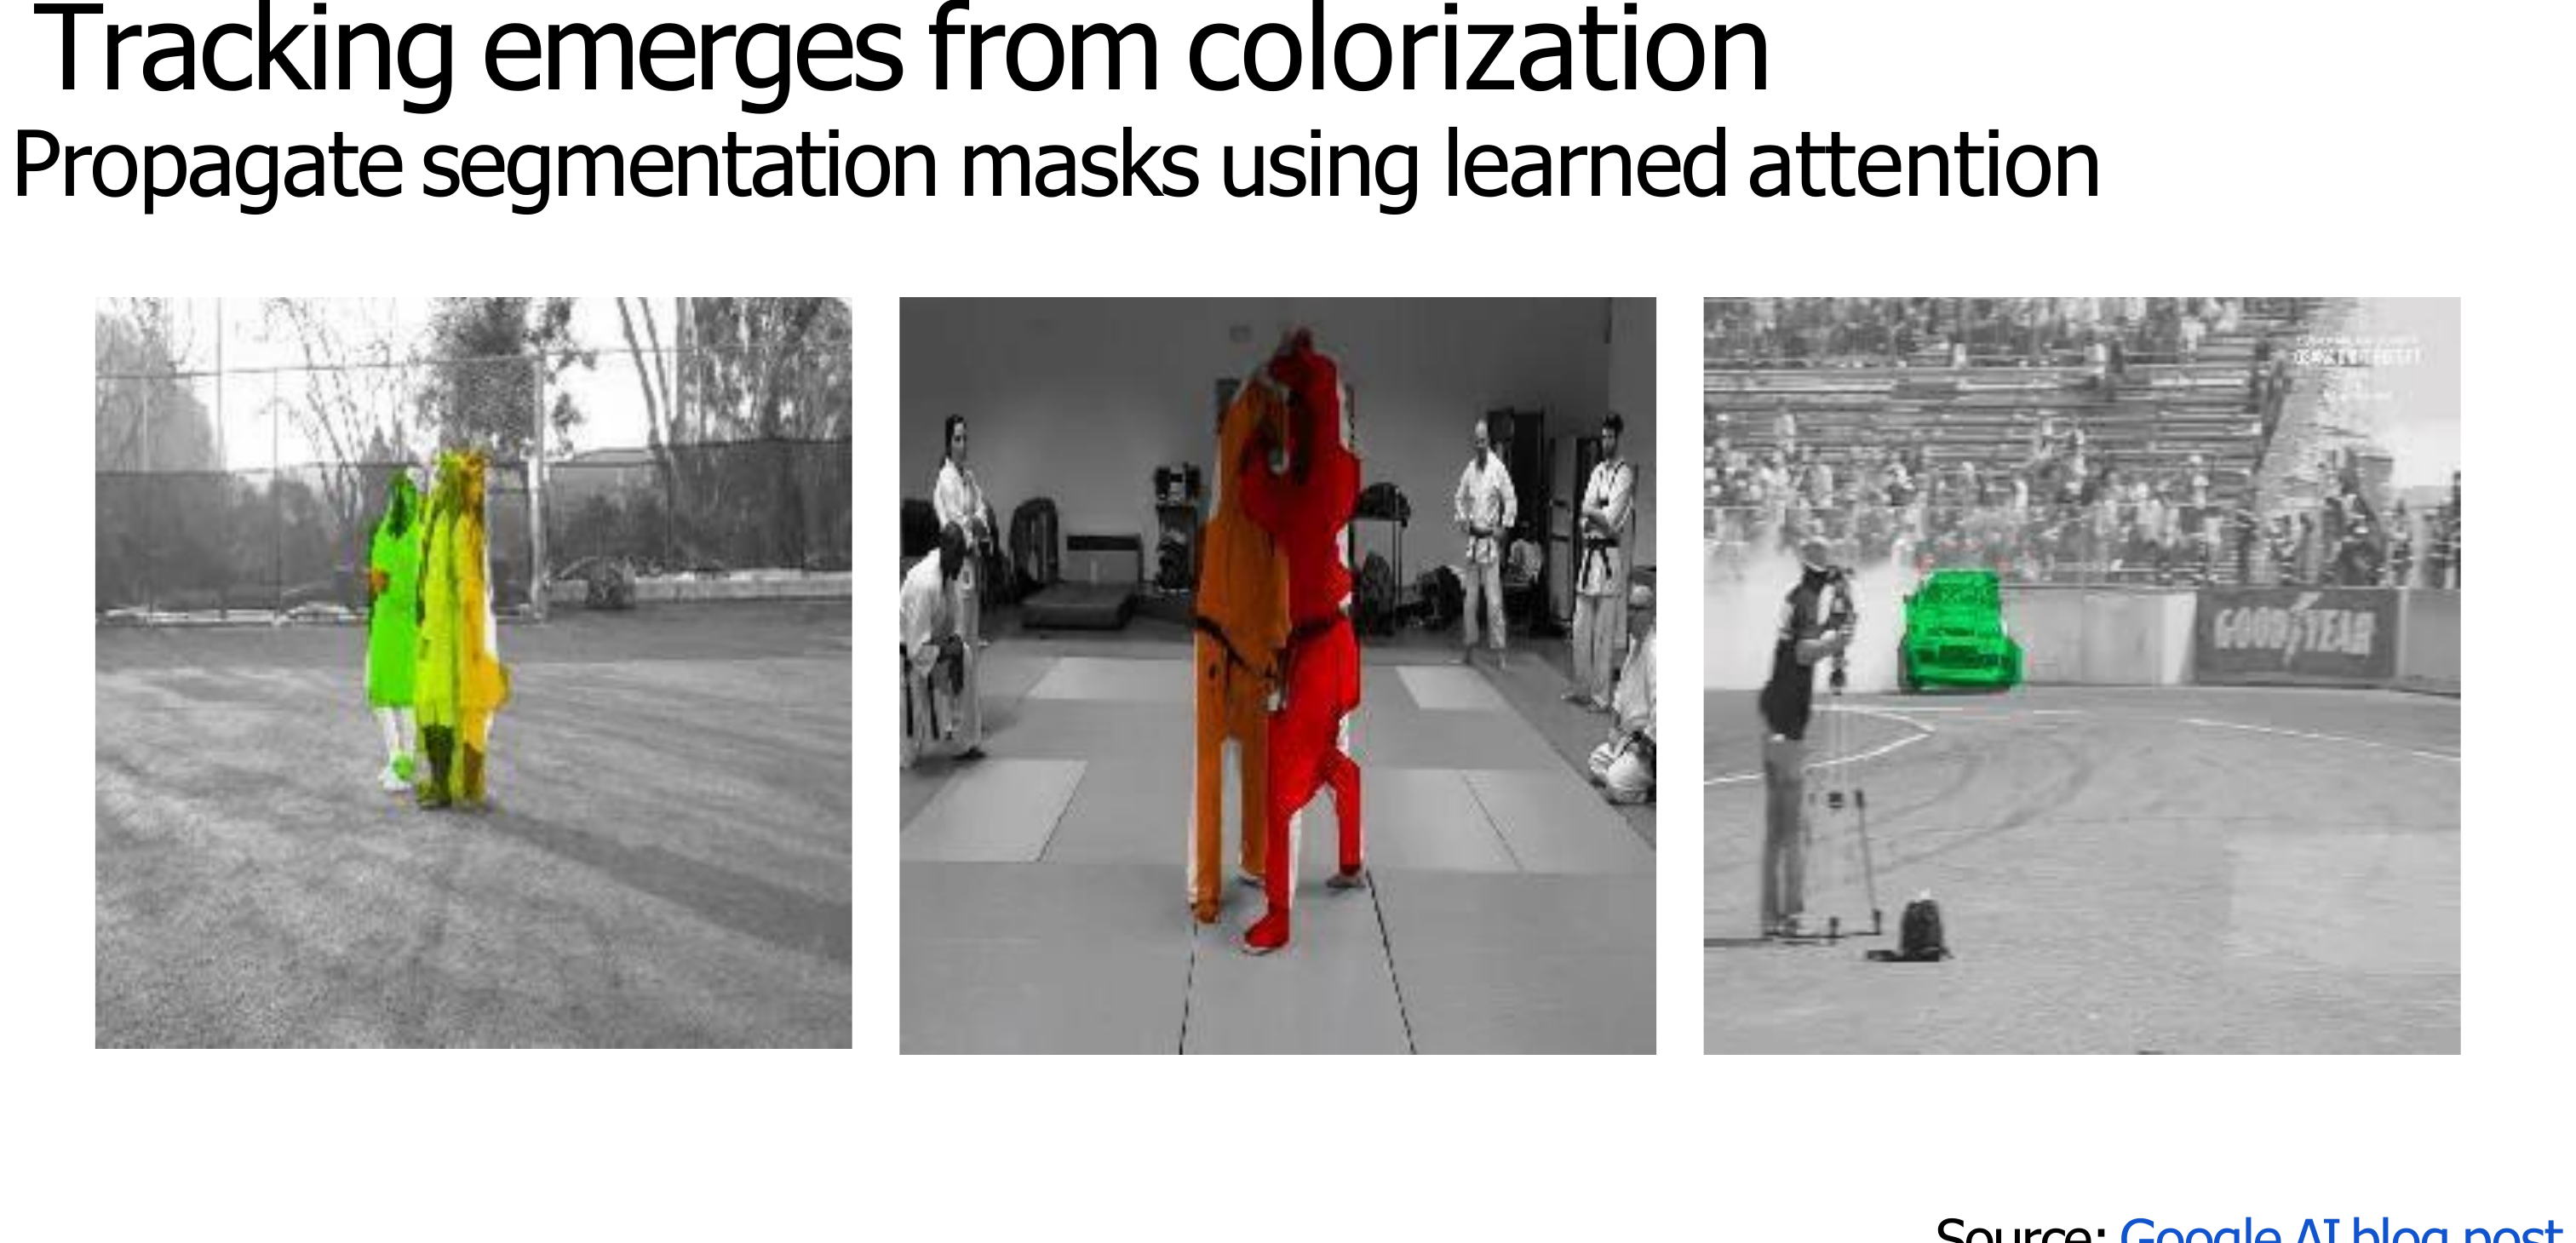
\includegraphics[width=0.88\textwidth]{Pictures/ssl_video_tracking_emergence.png}
    \caption{Emergent unsupervised tracking from video colorization (from course slides~\cite{galasso2025ssl, vondrick2018tracking}). Without human supervision, the attention weights learned to solve colorization automatically track semantic masks and human pose keypoints across frames.}\label{fig:ssl_video_tracking}
\end{figure}

\begin{InsightBox}
\textbf{Emergence of Tracking Without Human Labels:} \\
Because the only way to accurately colorize a moving object across video frames is to establish pixel-level correspondence, \textbf{visual object tracking emerges naturally as an unsupervised side-effect}. As shown in Figure~\ref{fig:ssl_video_tracking}, the learned attention matrix $A_{ij}$ successfully propagates semantic segmentation masks and human pose keypoints across time without any annotated training examples.
\end{InsightBox}

---

\section{Masked Autoencoders (MAE)}

\subsection{From Convolutional Inpainting to Vision Transformers}

While early context encoders operated on convolutional networks with small masked regions ($20\%$--$30\%$), He et al.~\cite{he2022masked} introduced \textbf{Masked Autoencoders (MAE)}, adapting BERT-style masked modeling~\cite{devlin2019bert} to the Vision Transformer (ViT) architecture.

\begin{figure}[htbp]
    \centering
    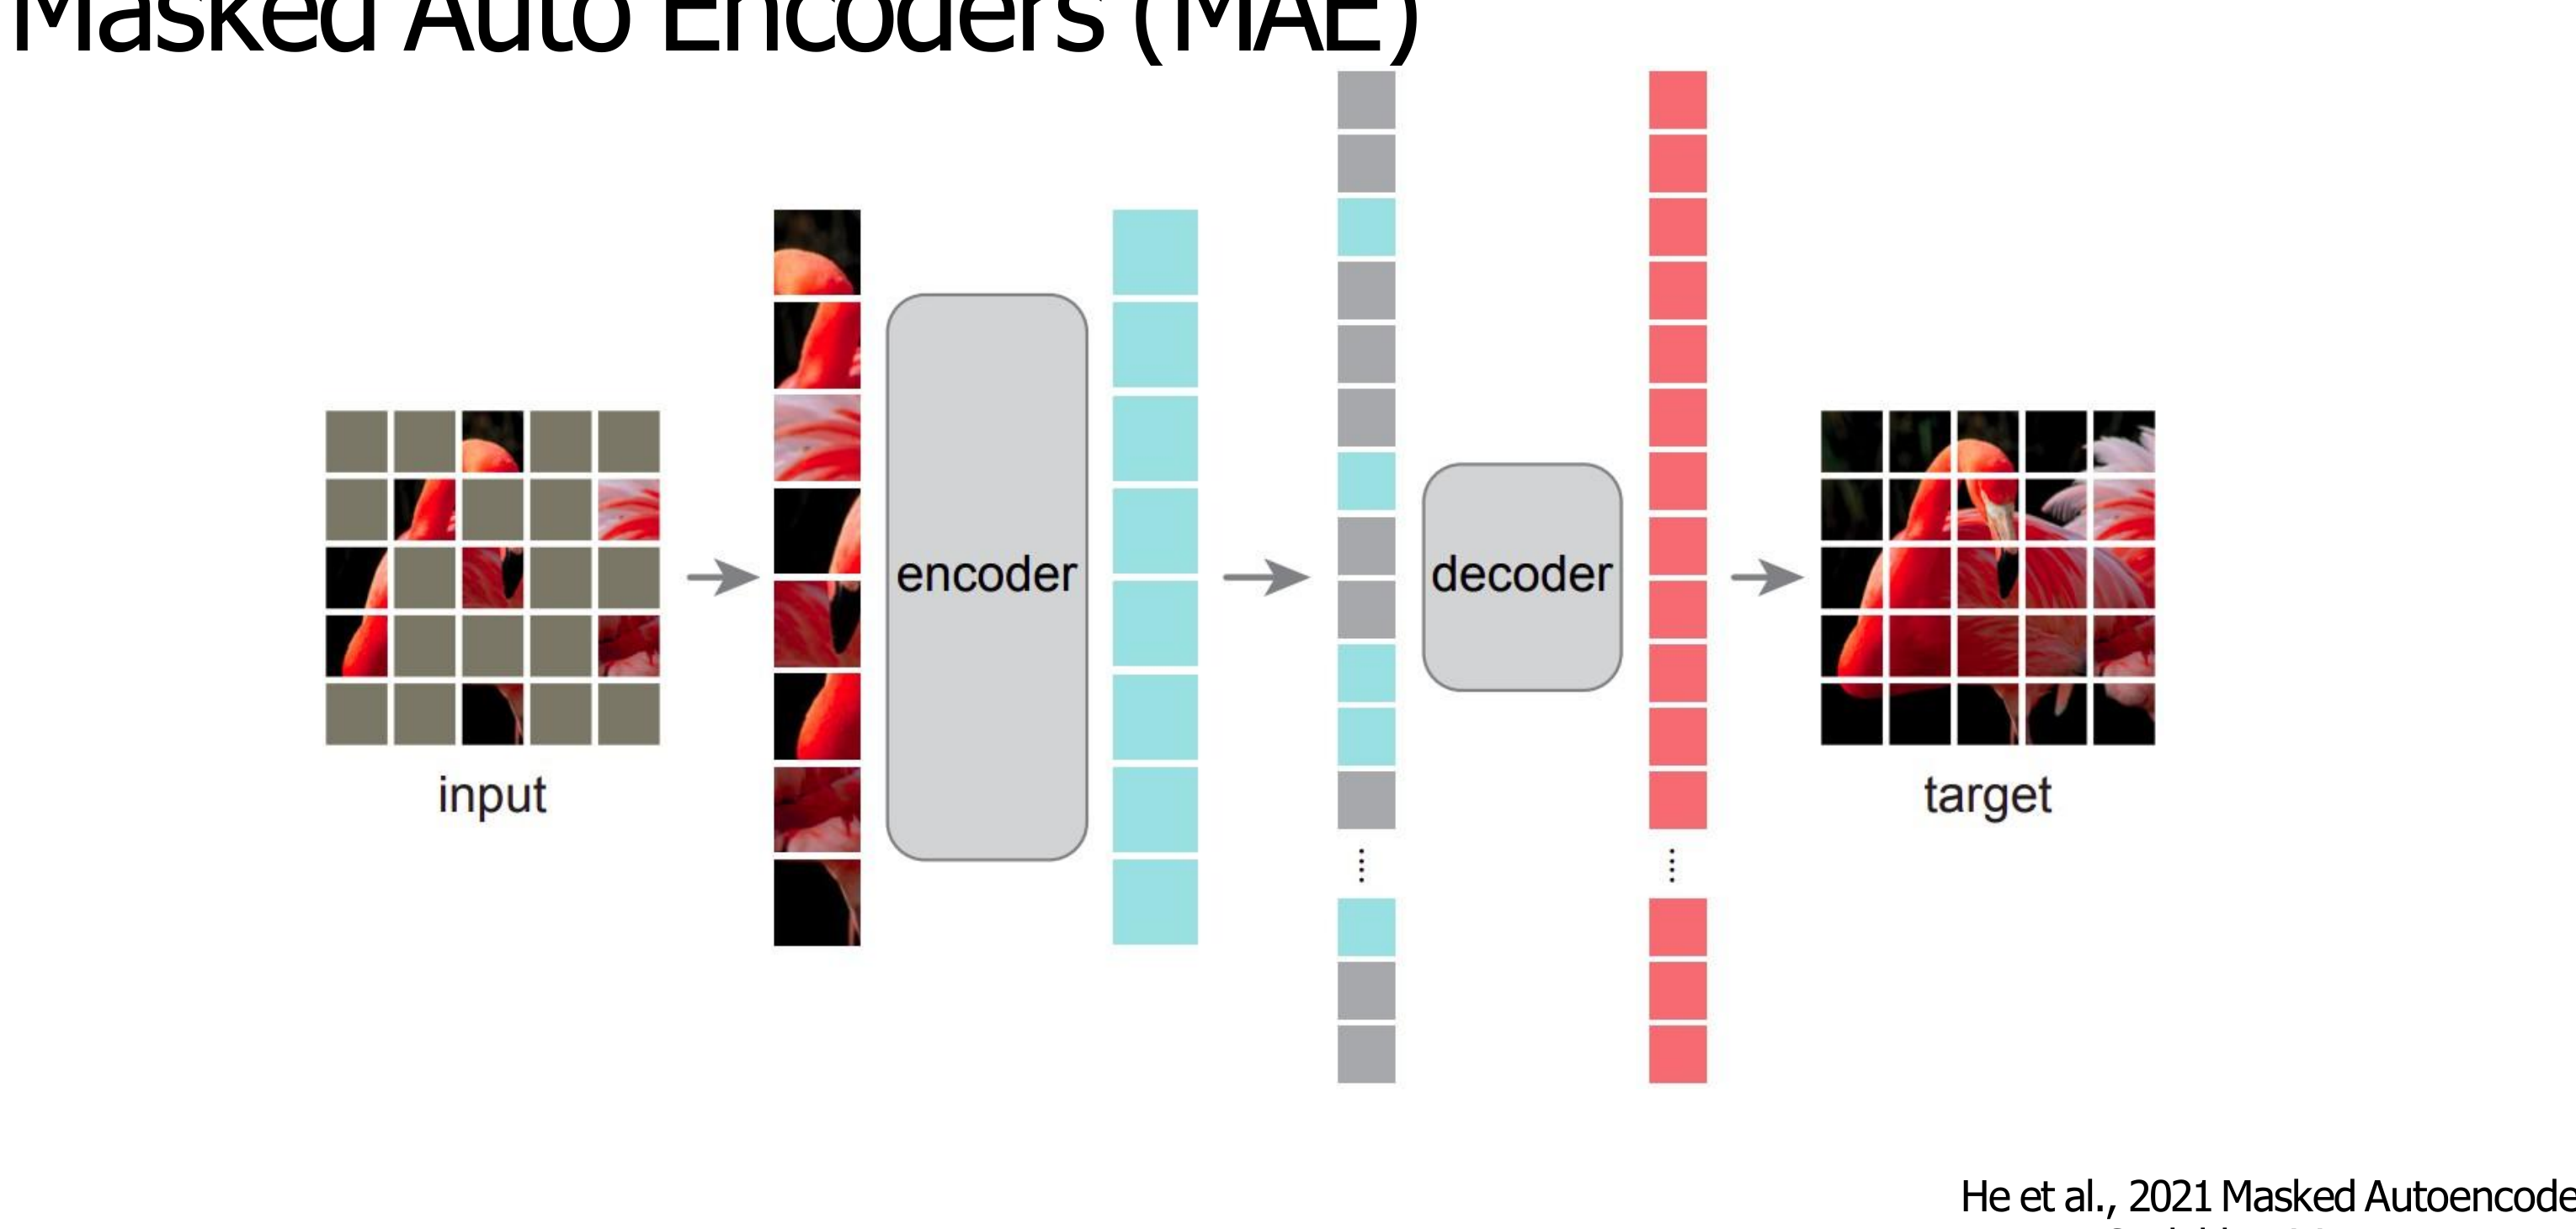
\includegraphics[width=0.92\textwidth]{Pictures/ssl_mae_architecture.png}
    \caption{Masked Autoencoders (MAE) architecture (from course slides~\cite{galasso2025ssl, he2022masked}). Left: ViT Encoder processes exclusively the visible patches ($25\%$). Right: A lightweight ViT Decoder merges encoded representations with shared learnable \texttt{[mask]} tokens to reconstruct pixel values.}\label{fig:ssl_mae_architecture}
\end{figure}

MAE builds upon a critical insight distinguishing vision from natural language:
\begin{itemize}[leftmargin=*]
    \item In language, words are highly semantic, information-dense symbols; masking $15\%$ of tokens creates an intellectually demanding completion task.
    \item In vision, images are continuous signals with \textbf{heavy spatial redundancy}. A patch can easily be interpolated from adjacent pixels without high-level semantic reasoning.
    \item \textbf{The Solution:} An \textbf{extreme masking ratio of $75\%$ to $80\%$}. At $75\%$ masking, neighboring information is stripped away, forcing the model to perform holistic holistic semantic scene understanding to synthesize plausible completions.
\end{itemize}

\subsection{The Asymmetric Encoder-Decoder Architecture}

The MAE architecture is uniquely asymmetric, consisting of two distinct stages:

\begin{enumerate}[leftmargin=*]
    \item \textbf{ViT Encoder (Visible Patches Only):} The original image is partitioned into non-overlapping patches (e.g., $16 \times 16$). A uniform random sample of $75\%$ of the patches is completely removed. Crucially, the deep ViT encoder operates \textbf{only on the remaining $25\%$ visible patches}. Because self-attention complexity scales quadratically with sequence length $N$ ($\mathcal{O}(N^2)$), dropping $75\%$ of tokens accelerates encoder training by more than an order of magnitude.
    \item \textbf{ViT Decoder (Full Token Sequence):} The decoder is a lightweight Transformer stack. Its input is the full sequence of tokens: the transformed representations of visible patches merged with shared, learnable \texttt{[mask]} tokens at the missing patch positions. Fixed sinusoidal positional embeddings are added to all tokens before decoding.
\end{enumerate}

\subsection{Reconstruction Objective and Normalization}

The decoder terminates in a linear projection layer that outputs pixel values for each masked patch. The network optimizes the Mean Squared Error (MSE) computed \textbf{exclusively on the masked patches}:
\begin{equation}
    \mathcal{L}_{\text{MAE}} = \frac{1}{|M|} \sum_{i \in M} \|x_i - \hat{x}_i\|_2^2
\end{equation}
where $M$ denotes the set of masked patch indices.

\begin{Notebox}
\textbf{Per-Patch Normalized Reconstruction:} \\
He et al.\@ demonstrated that normalizing each patch's raw pixel values by its local mean and standard deviation:
\begin{equation}
    x_i' = \frac{x_i - \mu_i}{\sigma_i + \epsilon}
\end{equation}
substantially boosts representation quality. Normalization forces the model to encode geometric shape, boundaries, and textures rather than trivial global illumination and contrast shifts.
\end{Notebox}

\subsection{Linear Probing vs.\ Fine-Tuning in Generative SSL}

A defining empirical hallmark of MAE (and masked modeling in general) is the divergence between linear probing and fine-tuning:
\begin{itemize}[leftmargin=*]
    \item \textbf{Linear Probing:} MAE representations achieve modest linear probing accuracy ($\approx 65\%$--$70\%$ on ImageNet). Because generative pixel reconstruction optimizes for low-level visual fidelity, semantic features are distributed across multiple layers rather than linearly separated at the final layer.
    \item \textbf{End-to-End Fine-Tuning:} When fine-tuned end-to-end, MAE achieves top-tier results ($87.8\%$ on ImageNet-1K with ViT-Huge), demonstrating that the weights serve as an exceptional general-purpose visual prior.
\end{itemize}

---

\section{Contrastive Representation Learning}

\subsection{Instance Discrimination and Hyperspherical Geometry}

While heuristic pretext tasks depend on hand-crafted spatial tricks, \textbf{Contrastive Representation Learning} establishes a principled, task-agnostic paradigm: \textbf{Instance Discrimination}. 

Every individual image is treated as its own discrete class. Given an image $x$, data augmentations generate correlated views $x^+$ (\emph{positive pair}). All other distinct images in the dataset $\{x_1^-, x_2^-, \dots\}$ serve as \emph{negative samples}. The objective is to map representations to a unit hypersphere $\mathbb{S}^{d-1}$ such that:
\begin{align}
    \text{sim}(f(x), f(x^+)) &\to 1 \quad &\text{(Attract positive views)} \\
    \text{sim}(f(x), f(x^-)) &\to -1 \quad &\text{(Repel negative instances)}
\end{align}

\subsection{The InfoNCE Loss Formulation}

Van den Oord et al.~\cite{oord2018representation} formalized contrastive learning via the \textbf{InfoNCE loss}. Given a query anchor representation $q$, a positive key $k^+$, and a dictionary of $K$ negative keys $\{k_1^-, \dots, k_K^-\}$, the loss is defined as:
\begin{equation}
    \mathcal{L}_{\text{InfoNCE}} = - \log \frac{\exp(\text{sim}(q, k^+) / \tau)}{\exp(\text{sim}(q, k^+) / \tau) + \sum_{j=1}^K \exp(\text{sim}(q, k_j^-) / \tau)}
\end{equation}
where $\text{sim}(u, v) = \frac{u^\top v}{\|u\|_2 \|v\|_2}$ denotes cosine similarity, and $\tau > 0$ is a temperature hyperparameter.

\begin{InsightBox}
\textbf{Connection to Cross-Entropy and Mutual Information:} \\
The InfoNCE loss is mathematically equivalent to the \textbf{multinomial cross-entropy loss of an $(K+1)$-way Softmax classifier} whose task is to correctly classify the positive sample among $K$ distractors. 

Furthermore, van den Oord et al.\@ proved that minimizing $\mathcal{L}_{\text{InfoNCE}}$ maximizes a rigorous \textbf{lower bound on the Mutual Information} $I(X; Y)$ between augmented views:
\begin{equation}
    I(X; Y) \ge \log(K + 1) - \mathcal{L}_{\text{InfoNCE}}
\end{equation}
A larger dictionary of negative keys $K$ tightens the mutual information bound, directly motivating architectures with massive negative sets.
\end{InsightBox}

\subsection{\texorpdfstring{SimCLR:\@ A Simple Framework for Contrastive Learning}{SimCLR (A Simple Framework for Contrastive Learning)}}

Chen et al.~\cite{chen2020simple} proposed \textbf{SimCLR}, formalizing four essential components of modern contrastive learning, as depicted in Figure~\ref{fig:ssl_simclr}:

\begin{figure}[htbp]
    \centering
    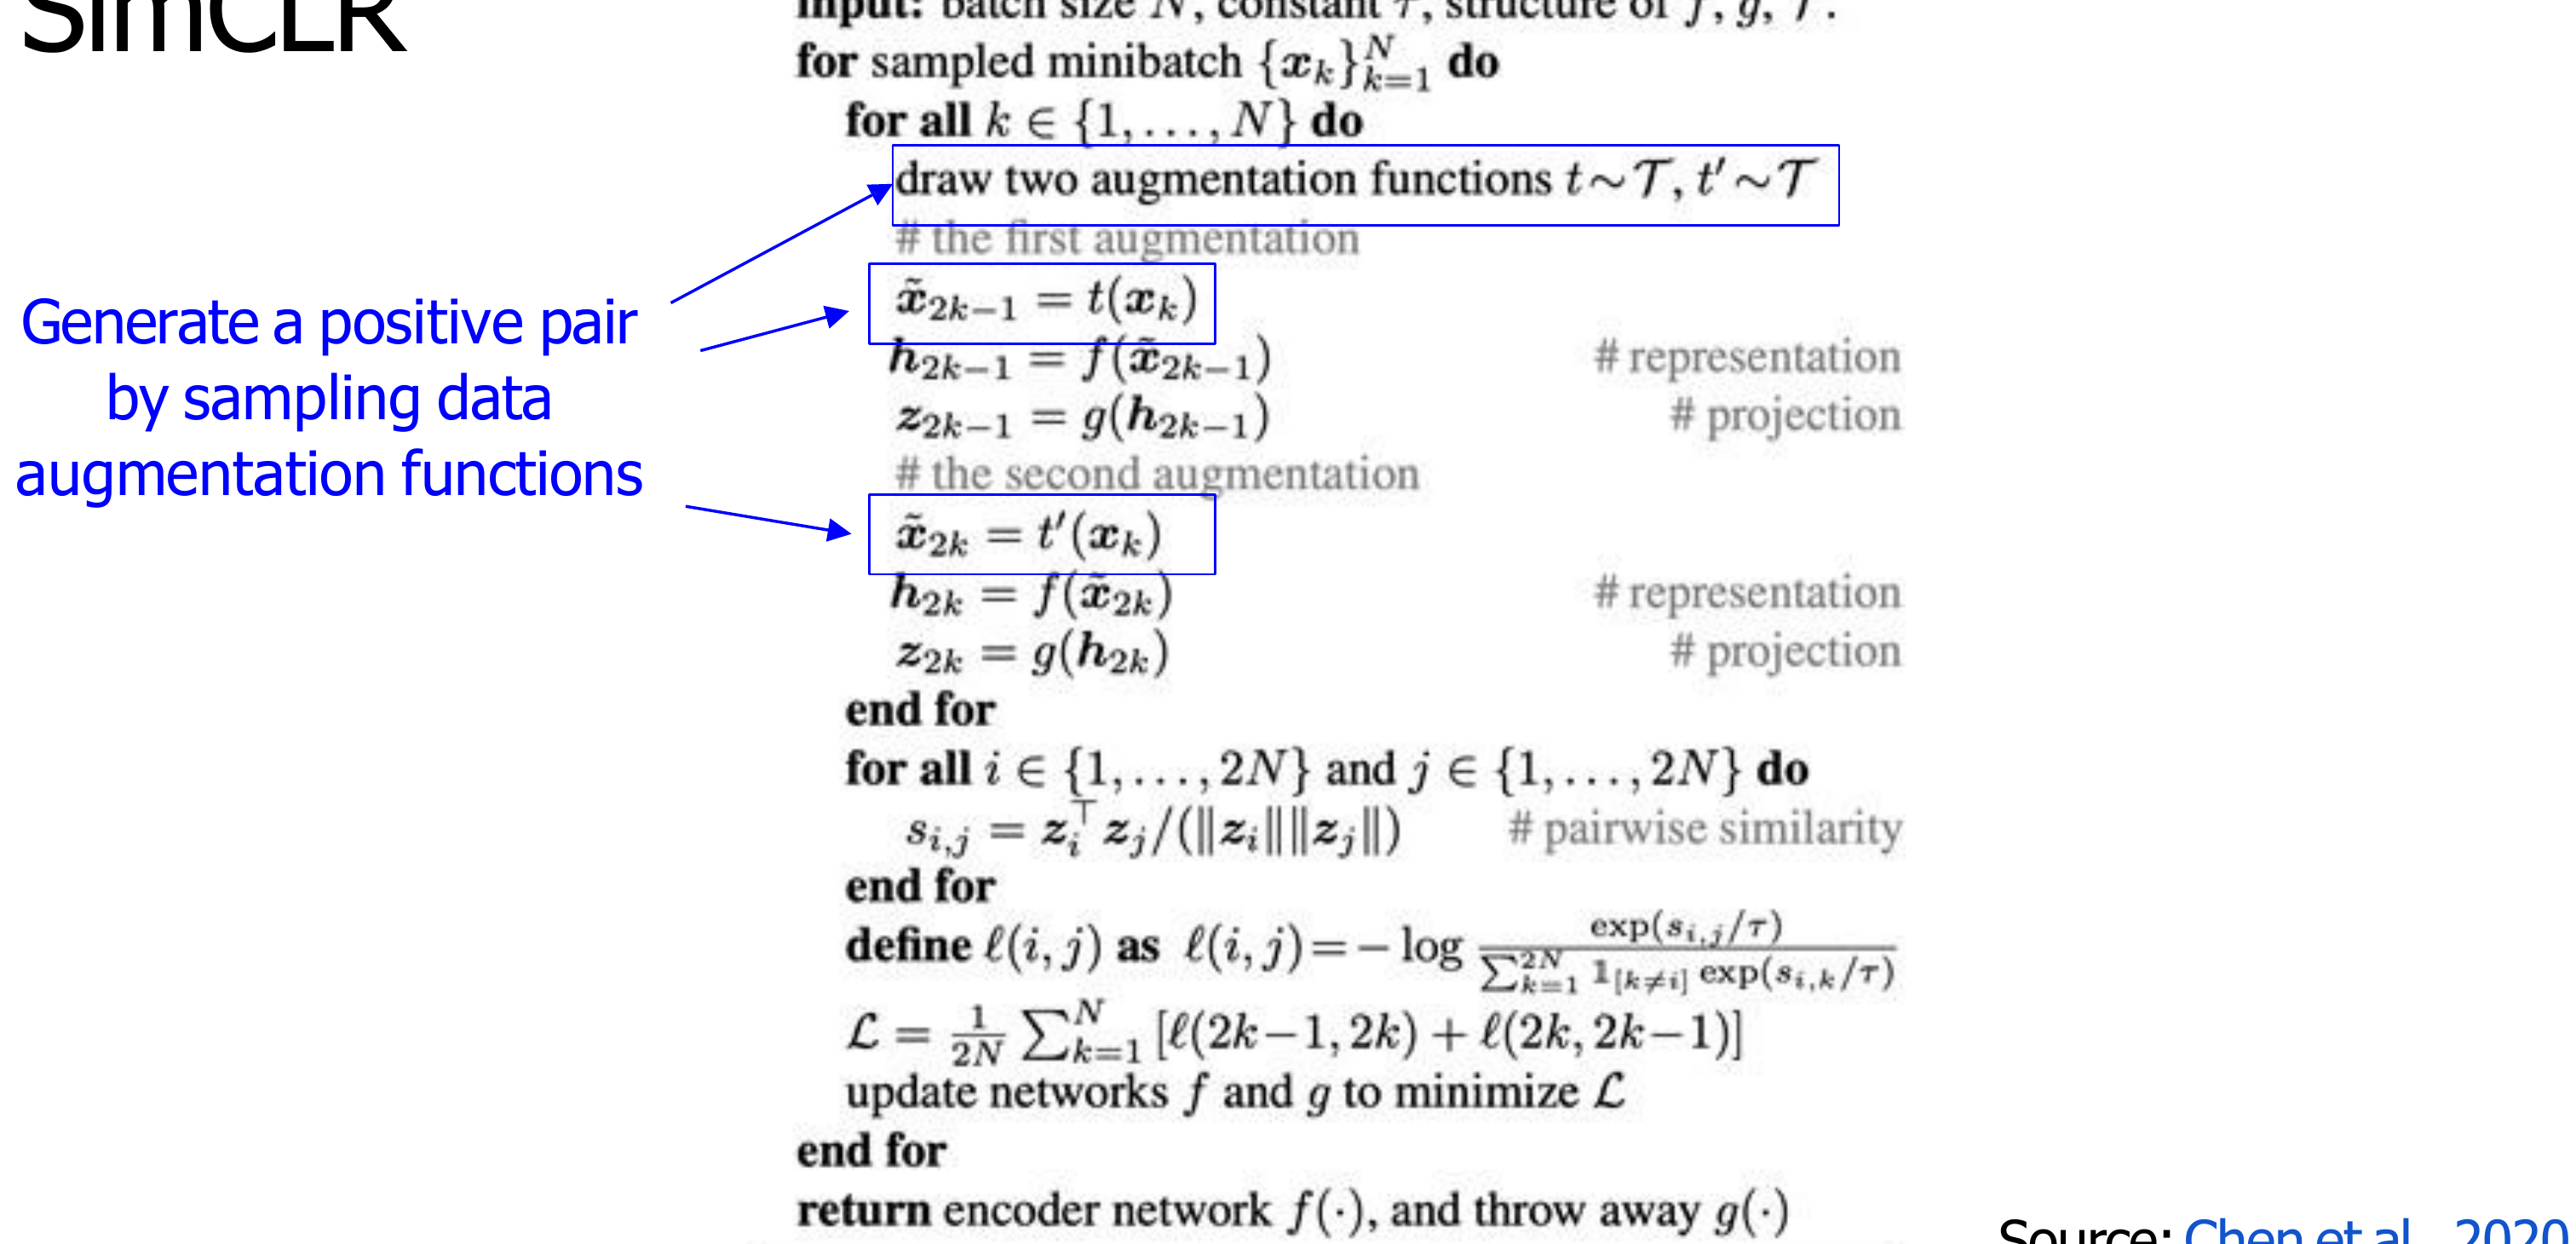
\includegraphics[width=0.90\textwidth]{Pictures/ssl_simclr_framework.png}
    \caption{The SimCLR framework (from course slides~\cite{galasso2025ssl, chen2020simple}). An image $x$ is transformed into two views $\tilde{x}_i, \tilde{x}_j$. A shared encoder $f(\cdot)$ extracts representations $h$, which are mapped by a non-linear projection head $g(\cdot)$ to space $z$ where the NT-Xent contrastive loss is evaluated.}\label{fig:ssl_simclr}
\end{figure}

\subsubsection{1. Composition of Data Augmentations}
Data augmentations define the invariance properties of the learned representation. SimCLR established that no single augmentation suffices; the critical synergy requires:
\begin{itemize}[leftmargin=*]
    \item \textbf{Random Crop and Resize:} Forces scale and spatial translation invariance.
    \item \textbf{Random Color Distortion (Color Jittering and Grayscale):} \textbf{Crucial safeguard!} Without color distortion, the model exploits 8-bit color histograms as a shortcut, matching views of the same image based on global tint rather than object geometry.
    \item \textbf{Gaussian Blur:} Removes high-frequency texture shortcuts.
\end{itemize}

\subsubsection{2. The Non-Linear Projection Head}
SimCLR maps encoder representations $h = f(x) \in \mathbb{R}^d$ through a small Multi-Layer Perceptron (MLP) \textbf{projection head}:
\begin{equation}
    z = g(h) = W^{(2)} \sigma(W^{(1)} h)
\end{equation}
The contrastive loss is applied on $z \in \mathbb{R}^{d'}$, but after pre-training, \textbf{the projection head $g(\cdot)$ is discarded}, and downstream tasks evaluate representations directly on $h$.

\begin{InsightBox}
\textbf{Why Discard the Projection Head?} \\
The contrastive objective forces $z$ to be strictly invariant to data augmentations (such as color shifts, scaling, and rotation). However, downstream tasks (e.g., fine-grained bird classification or bounding-box detection) often require precise color and spatial scale information! The intermediate representation $h$ preserves richer visual features that the non-linear projection layer strips out to minimize the contrastive objective on $z$.
\end{InsightBox}

\subsubsection{3. Normalized Temperature-Scaled Cross-Entropy (NT-Xent)}
In a mini-batch of $N$ images, data augmentation yields $2N$ views. For any positive pair $(i, j)$ derived from the same source image, the remaining $2(N - 1)$ augmented views in the mini-batch serve as negative samples:
\begin{equation}
    \ell_{i,j} = - \log \frac{\exp(\text{sim}(z_i, z_j) / \tau)}{\sum_{k=1}^{2N} \mathbb{I}_{[k \neq i]} \exp(\text{sim}(z_i, z_k) / \tau)}
\end{equation}
The total mini-batch loss is computed symmetrically across all $2N$ samples.

\subsubsection{4. Large Batch Dependency}
Because negatives are sourced strictly within the current mini-batch ($K = 2N - 2$), SimCLR requires massive batch sizes ($N = 2048$ to $4096$, providing $4094$ to $8190$ negatives) to achieve optimal performance, necessitating large TPU/GPU cluster parallelization.

\subsection{\texorpdfstring{Momentum Contrast (MoCo and MoCo v2)}{Momentum Contrast (MoCo and MoCo v2)}}

To overcome the large batch requirement of SimCLR, He et al.~\cite{he2020momentum} introduced \textbf{Momentum Contrast (MoCo)}, framing contrastive learning as a \textbf{continuous dictionary lookup}, shown in Figure~\ref{fig:ssl_moco}:

\begin{figure}[htbp]
    \centering
    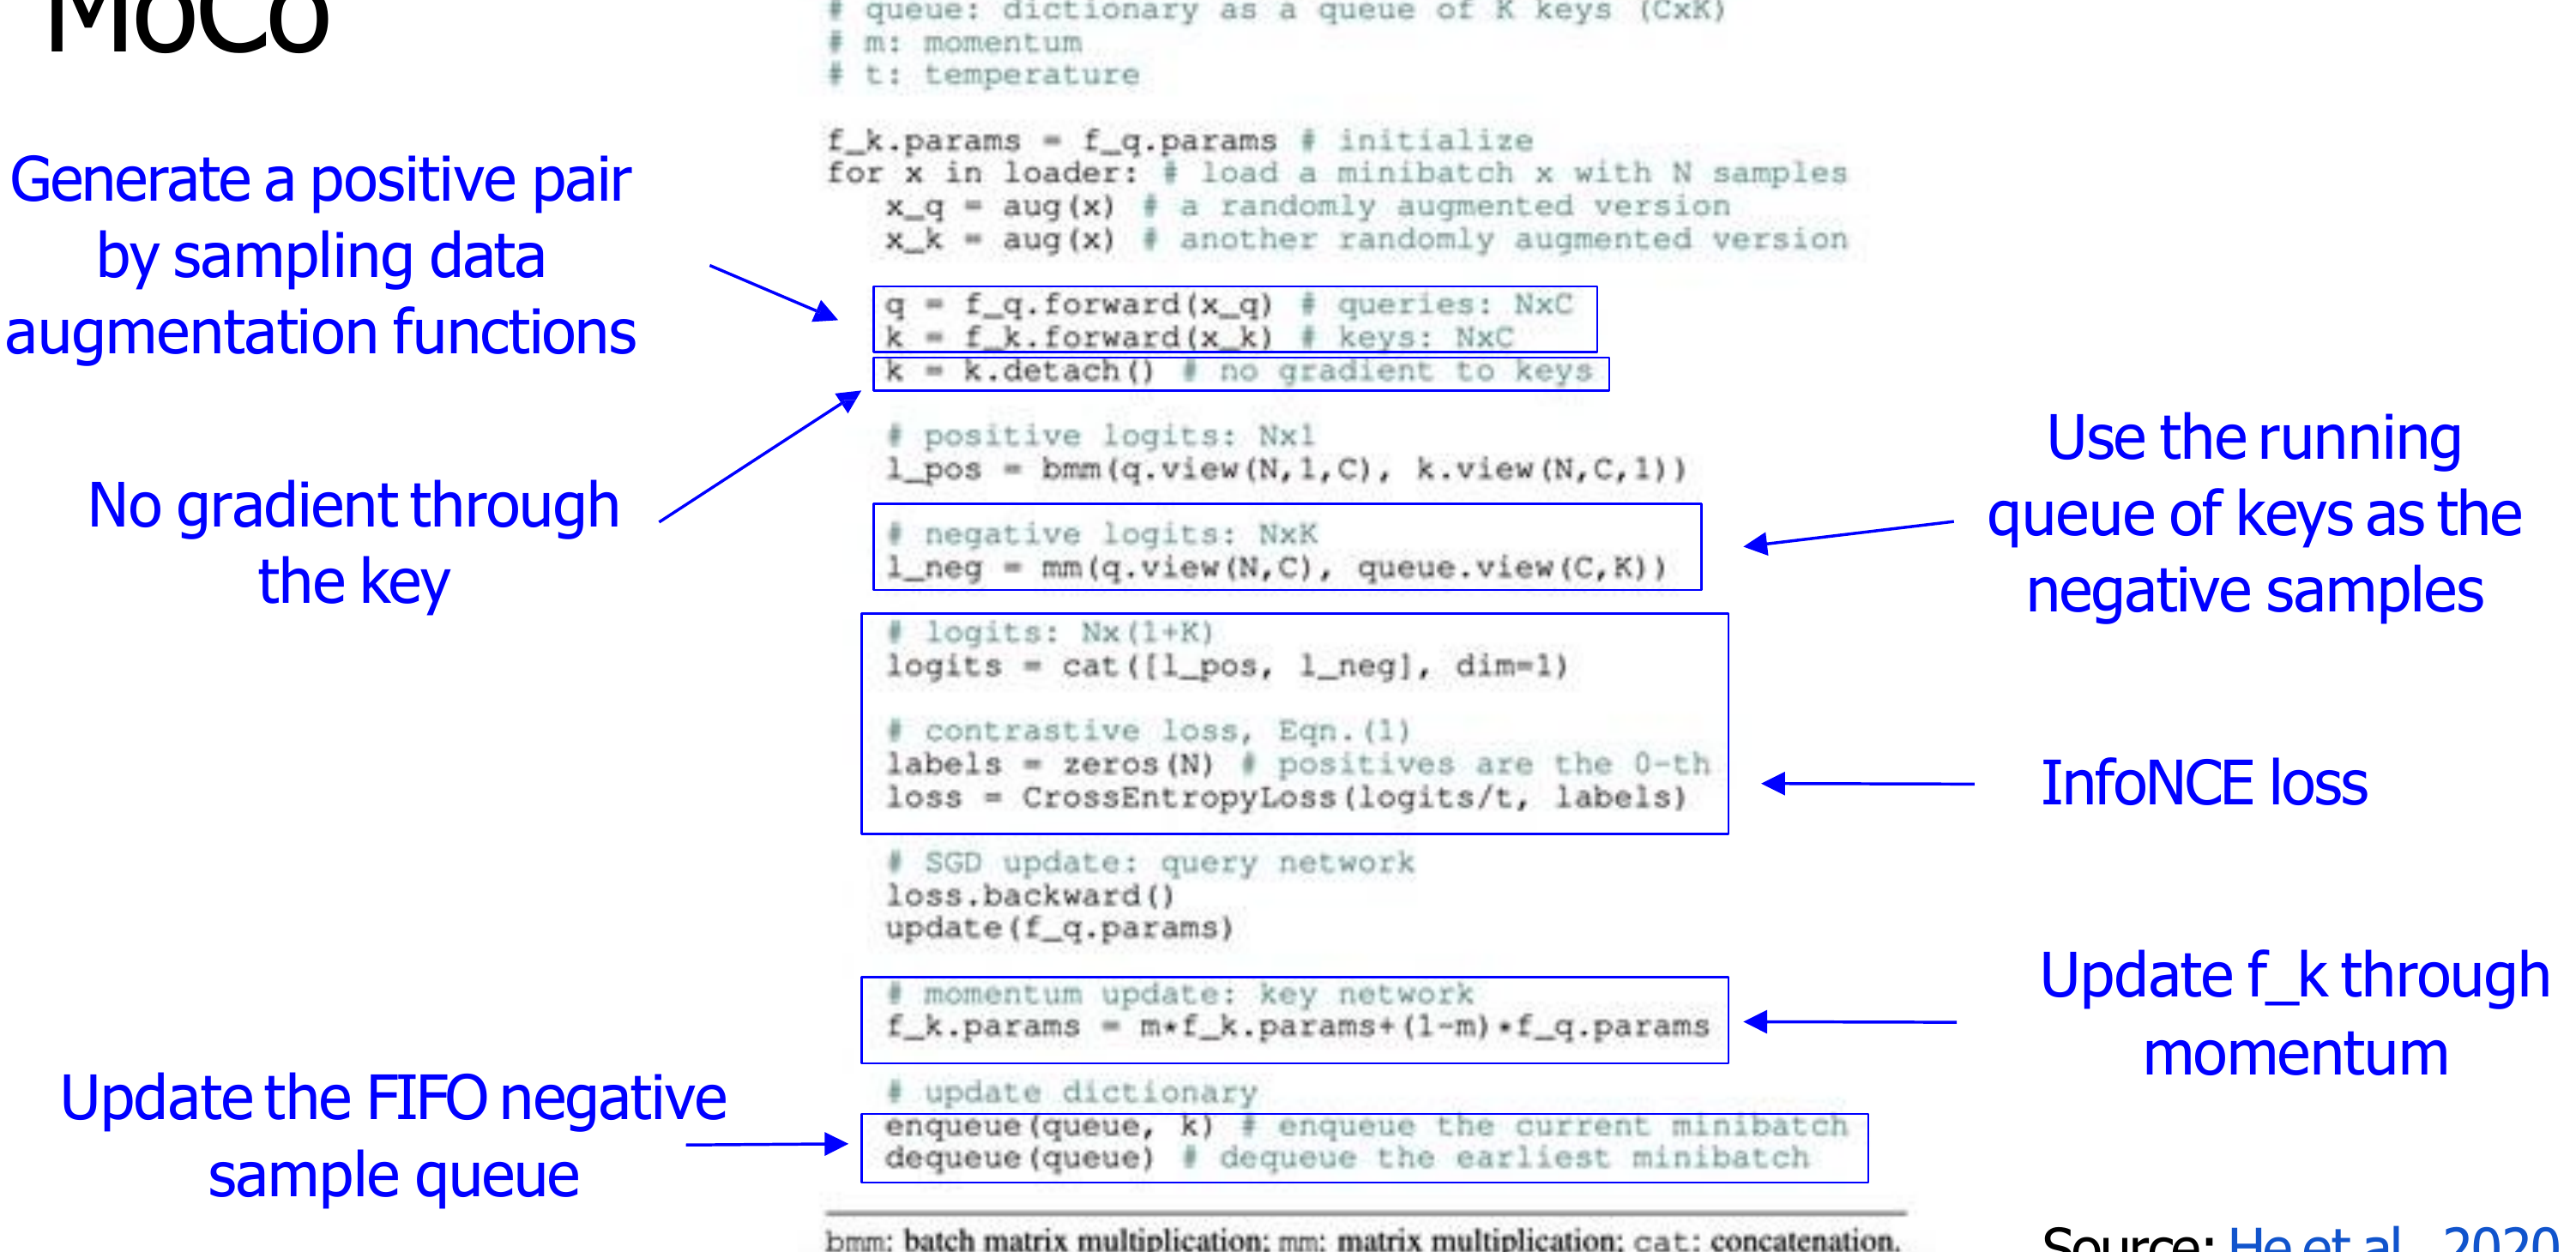
\includegraphics[width=0.90\textwidth]{Pictures/ssl_moco_framework_queue.png}
    \caption{The MoCo framework (from course slides~\cite{galasso2025ssl, he2020momentum}). A dynamic FIFO queue decouples negative dictionary size from mini-batch size. A momentum-updated key encoder ensures key representations remain temporally consistent without backpropagating through the entire queue.}\label{fig:ssl_moco}
\end{figure}

MoCo introduces two pivotal architectural mechanisms:
\begin{enumerate}[leftmargin=*]
    \item \textbf{Dynamic Memory Queue (Decoupling Dictionary Size):} Instead of sourcing negatives from the current mini-batch, MoCo maintains a large first-in, first-out (FIFO) queue of negative keys ($K = 65{,}536$). At each training step, the current mini-batch keys are enqueued, and the oldest keys are evicted. This decouples dictionary size $K$ from mini-batch size $N$, allowing massive negative dictionaries with a modest batch size ($N = 256$).
    \item \textbf{Momentum Encoder Update:} Backpropagating gradients through $65{,}536$ historical keys stored in memory is computationally intractable. However, updating the key encoder weights $\theta_k$ directly via SGD causes catastrophic feature drift: keys enqueued at step $t - 100$ were computed with an obsolete encoder and are inconsistent with current query representations.
\end{enumerate}

MoCo solves feature consistency by updating the Key Encoder $\theta_k$ via an \textbf{Exponential Moving Average (EMA)} of the Query Encoder $\theta_q$:
\begin{equation}
    \theta_k \leftarrow m \, \theta_k + (1 - m) \, \theta_q
\end{equation}
where $m \approx 0.999$ is a momentum coefficient. The query encoder $\theta_q$ is updated by backpropagation; the key encoder $\theta_k$ receives \textbf{no direct gradients}. The slow, smooth momentum evolution ensures that keys across the $65{,}536$-sample queue remain mutually consistent.

Chen et al.~\cite{chen2020improved} subsequently released \textbf{MoCo v2}, integrating SimCLR's non-linear projection head and cosine learning rate decay into the MoCo framework. MoCo v2 surpassed SimCLR while running on standard, affordable GPU hardware without requiring multi-node TPU pods.

---

\section{Non-Contrastive Siamese Architectures}

\subsection{The Representation Collapse Problem}

In contrastive learning, negative pairs supply the repulsive force that prevents \textbf{representation collapse}---the degenerate failure mode where all images map to an identical, constant output vector $f(x) = c$.

However, maintaining thousands of negative samples introduces substantial memory and computational overhead. Can a Siamese network learn high-quality representations \textbf{without any negative samples}?

\subsection{\texorpdfstring{BYOL:\@ Bootstrap Your Own Latent}{BYOL (Bootstrap Your Own Latent)}}

Grill et al.~\cite{grill2020bootstrap} demonstrated that negative samples are not required if the network introduces \textbf{architectural asymmetry}. The resulting method, \textbf{Bootstrap Your Own Latent (BYOL)}, is illustrated in Figure~\ref{fig:ssl_byol}:

\begin{figure}[htbp]
    \centering
    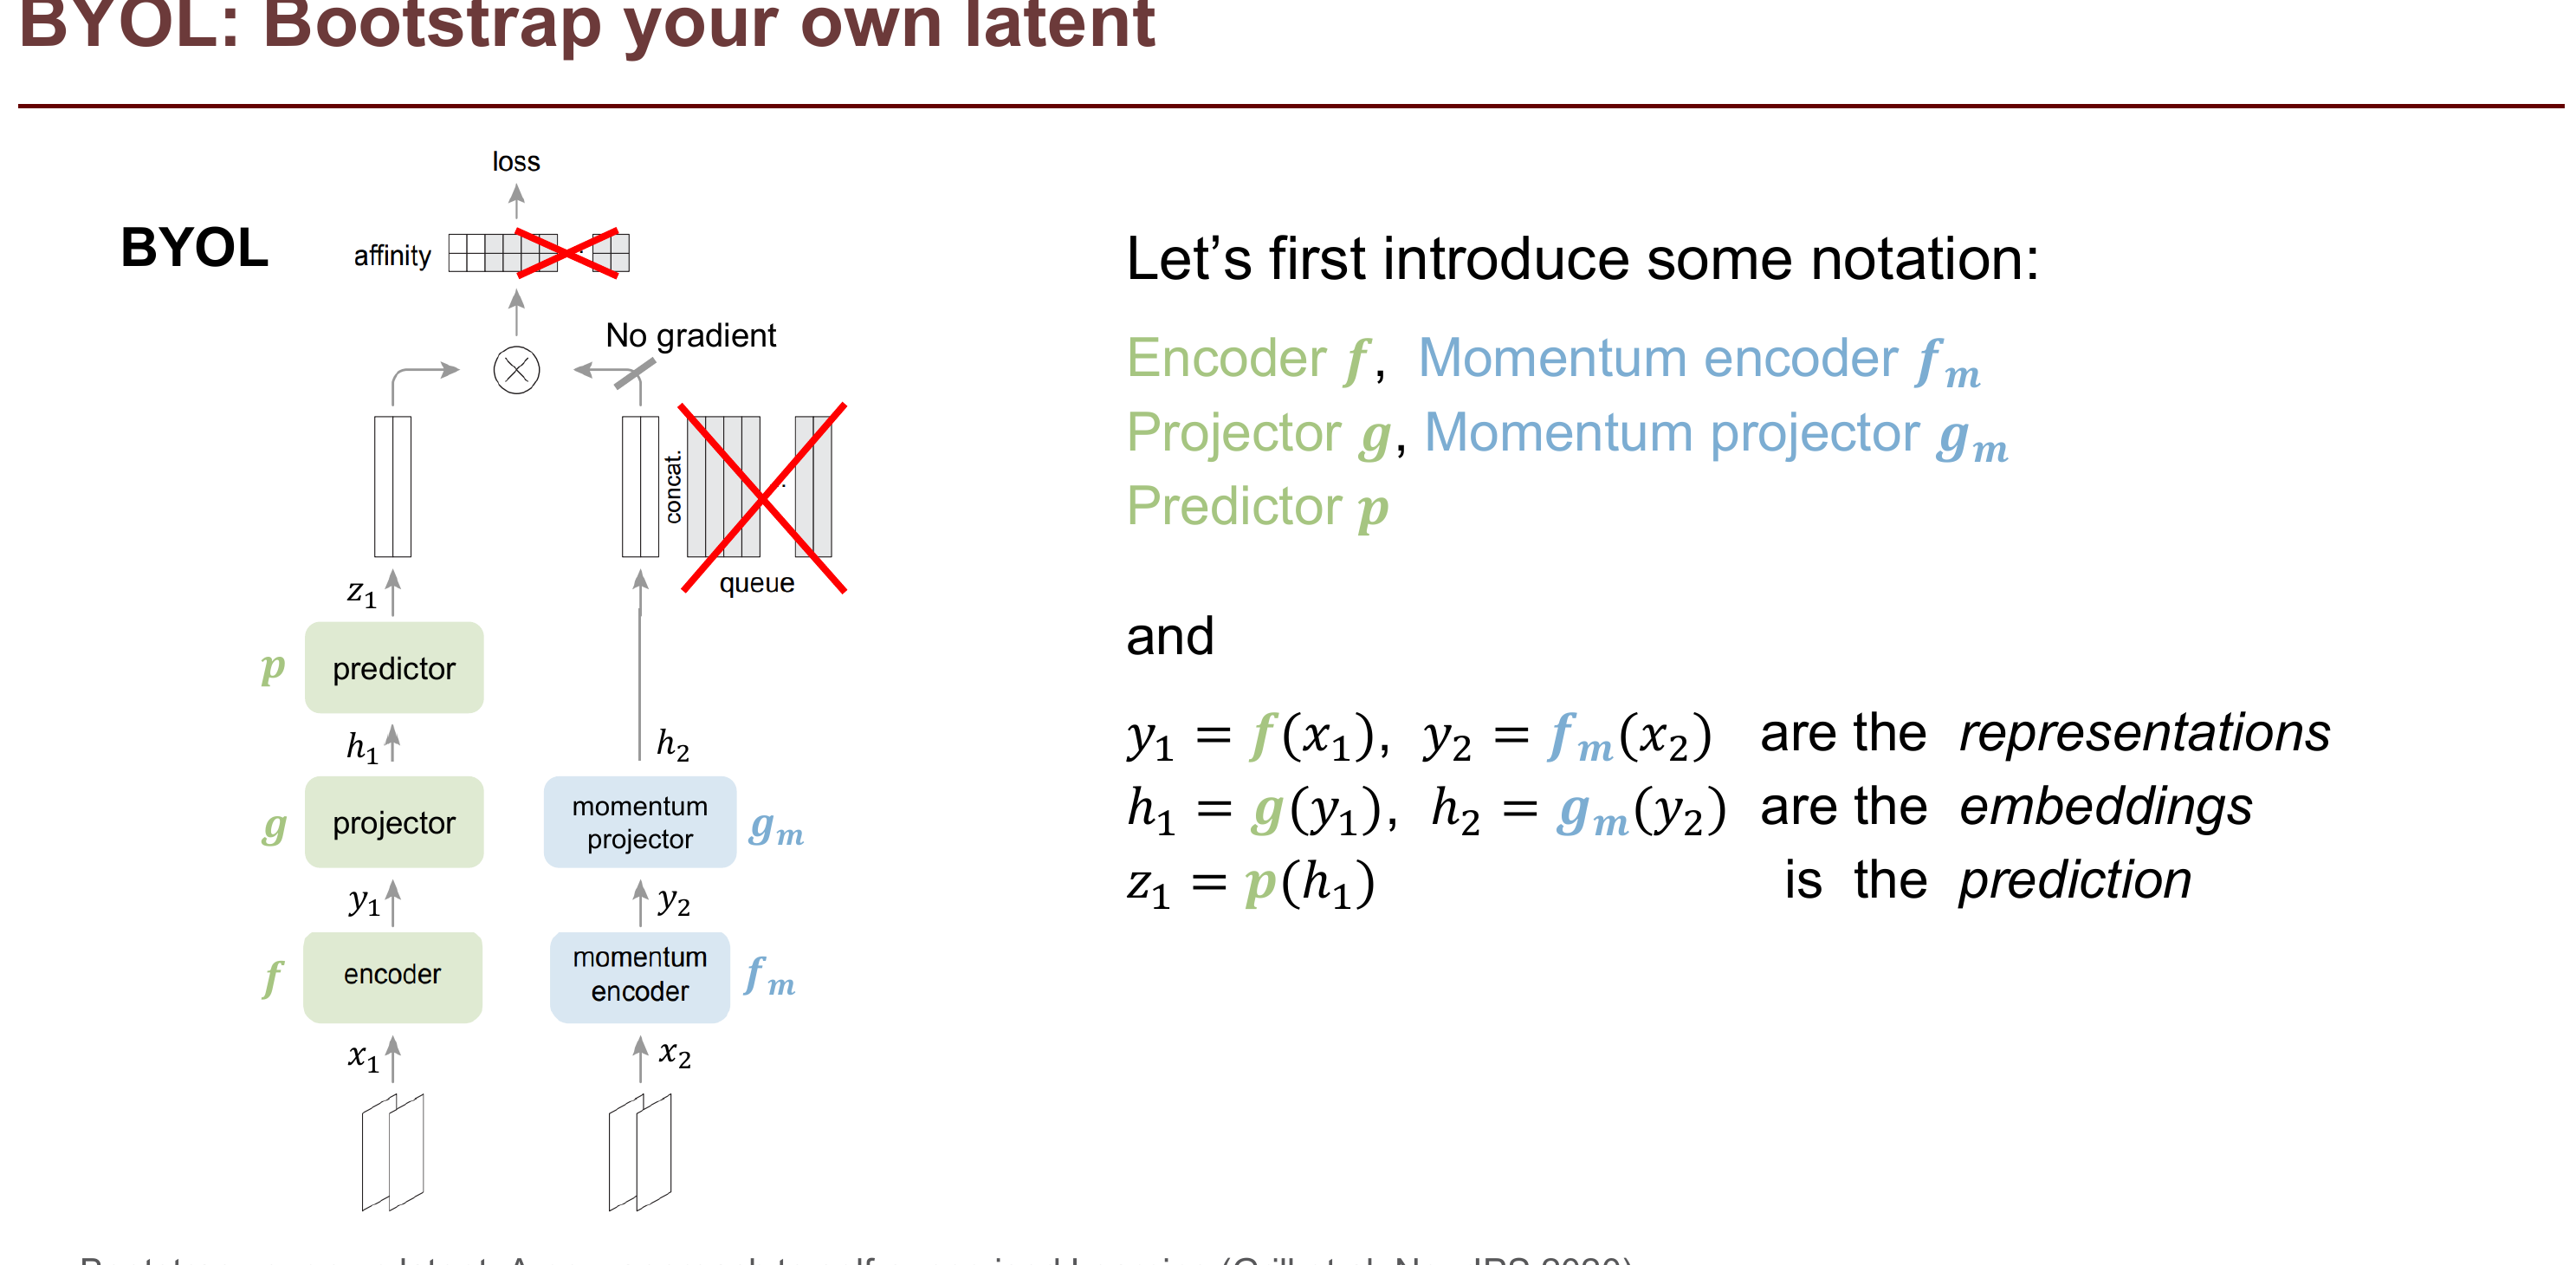
\includegraphics[width=0.90\textwidth]{Pictures/ssl_byol_architecture.png}
    \caption{The BYOL architecture (from course slides~\cite{galasso2025ssl, grill2020bootstrap}). BYOL eliminates negative pairs entirely by coupling an online network (with an additional predictor head) to an EMA target network with a stop-gradient operator.}\label{fig:ssl_byol}
\end{figure}

BYOL partitions computation between two asymmetric branches:
\begin{itemize}[leftmargin=*]
    \item \textbf{Online Network ($\theta$):} Comprises an encoder $f_\theta$, a projector $g_\theta$, and an additional \textbf{predictor head} $q_\theta$:
    \begin{equation}
        y_1 = f_\theta(x_1), \quad z_1 = g_\theta(y_1), \quad p_1 = q_\theta(z_1)
    \end{equation}
    \item \textbf{Target Network ($\xi$):} Comprises an encoder $f_\xi$ and projector $g_\xi$, but \textbf{no predictor head}:
    \begin{equation}
        y_2 = f_\xi(x_2), \quad z_2 = g_\xi(y_2)
    \end{equation}
    The target network parameters $\xi$ are updated via EMA:\@ $\xi \leftarrow \tau \xi + (1 - \tau)\theta$, and receive \textbf{no gradients} ($\text{stopgrad}$).
\end{itemize}

The loss is the Mean Squared Error between normalized predictions and normalized target projections:
\begin{equation}
    \mathcal{L}_{\text{BYOL}} = 2 - 2 \, \frac{\langle p_1, z_2 \rangle}{\|p_1\|_2 \|z_2\|_2}
\end{equation}
The loss is symmetrized by feeding $x_2$ to the online branch and $x_1$ to the target branch. 

\begin{InsightBox}
\textbf{Why Does BYOL Not Collapse?} \\
Collapse is prevented by the dynamic interplay between the predictor head and the EMA target network:
\begin{enumerate}
    \item The target network acts as an evolving, non-stationary regression target; the online network is constantly chasing a moving representation rather than a static point.
    \item The predictor $q_\theta$ breaks mathematical symmetry: the online network must predict the target representation from an augmented view, forcing the encoder to capture invariant semantic structure.
\end{enumerate}
\end{InsightBox}

\subsection{\texorpdfstring{SimSiam: Exploring Simple Siamese Representation Learning}{SimSiam: Exploring Simple Siamese Representation Learning}}

Chen and He~\cite{chen2021exploring} pushed non-contrastive simplification to its ultimate limit with \textbf{SimSiam (Simple Siamese)}, shown in Figure~\ref{fig:ssl_simsiam}:

\begin{figure}[htbp]
    \centering
    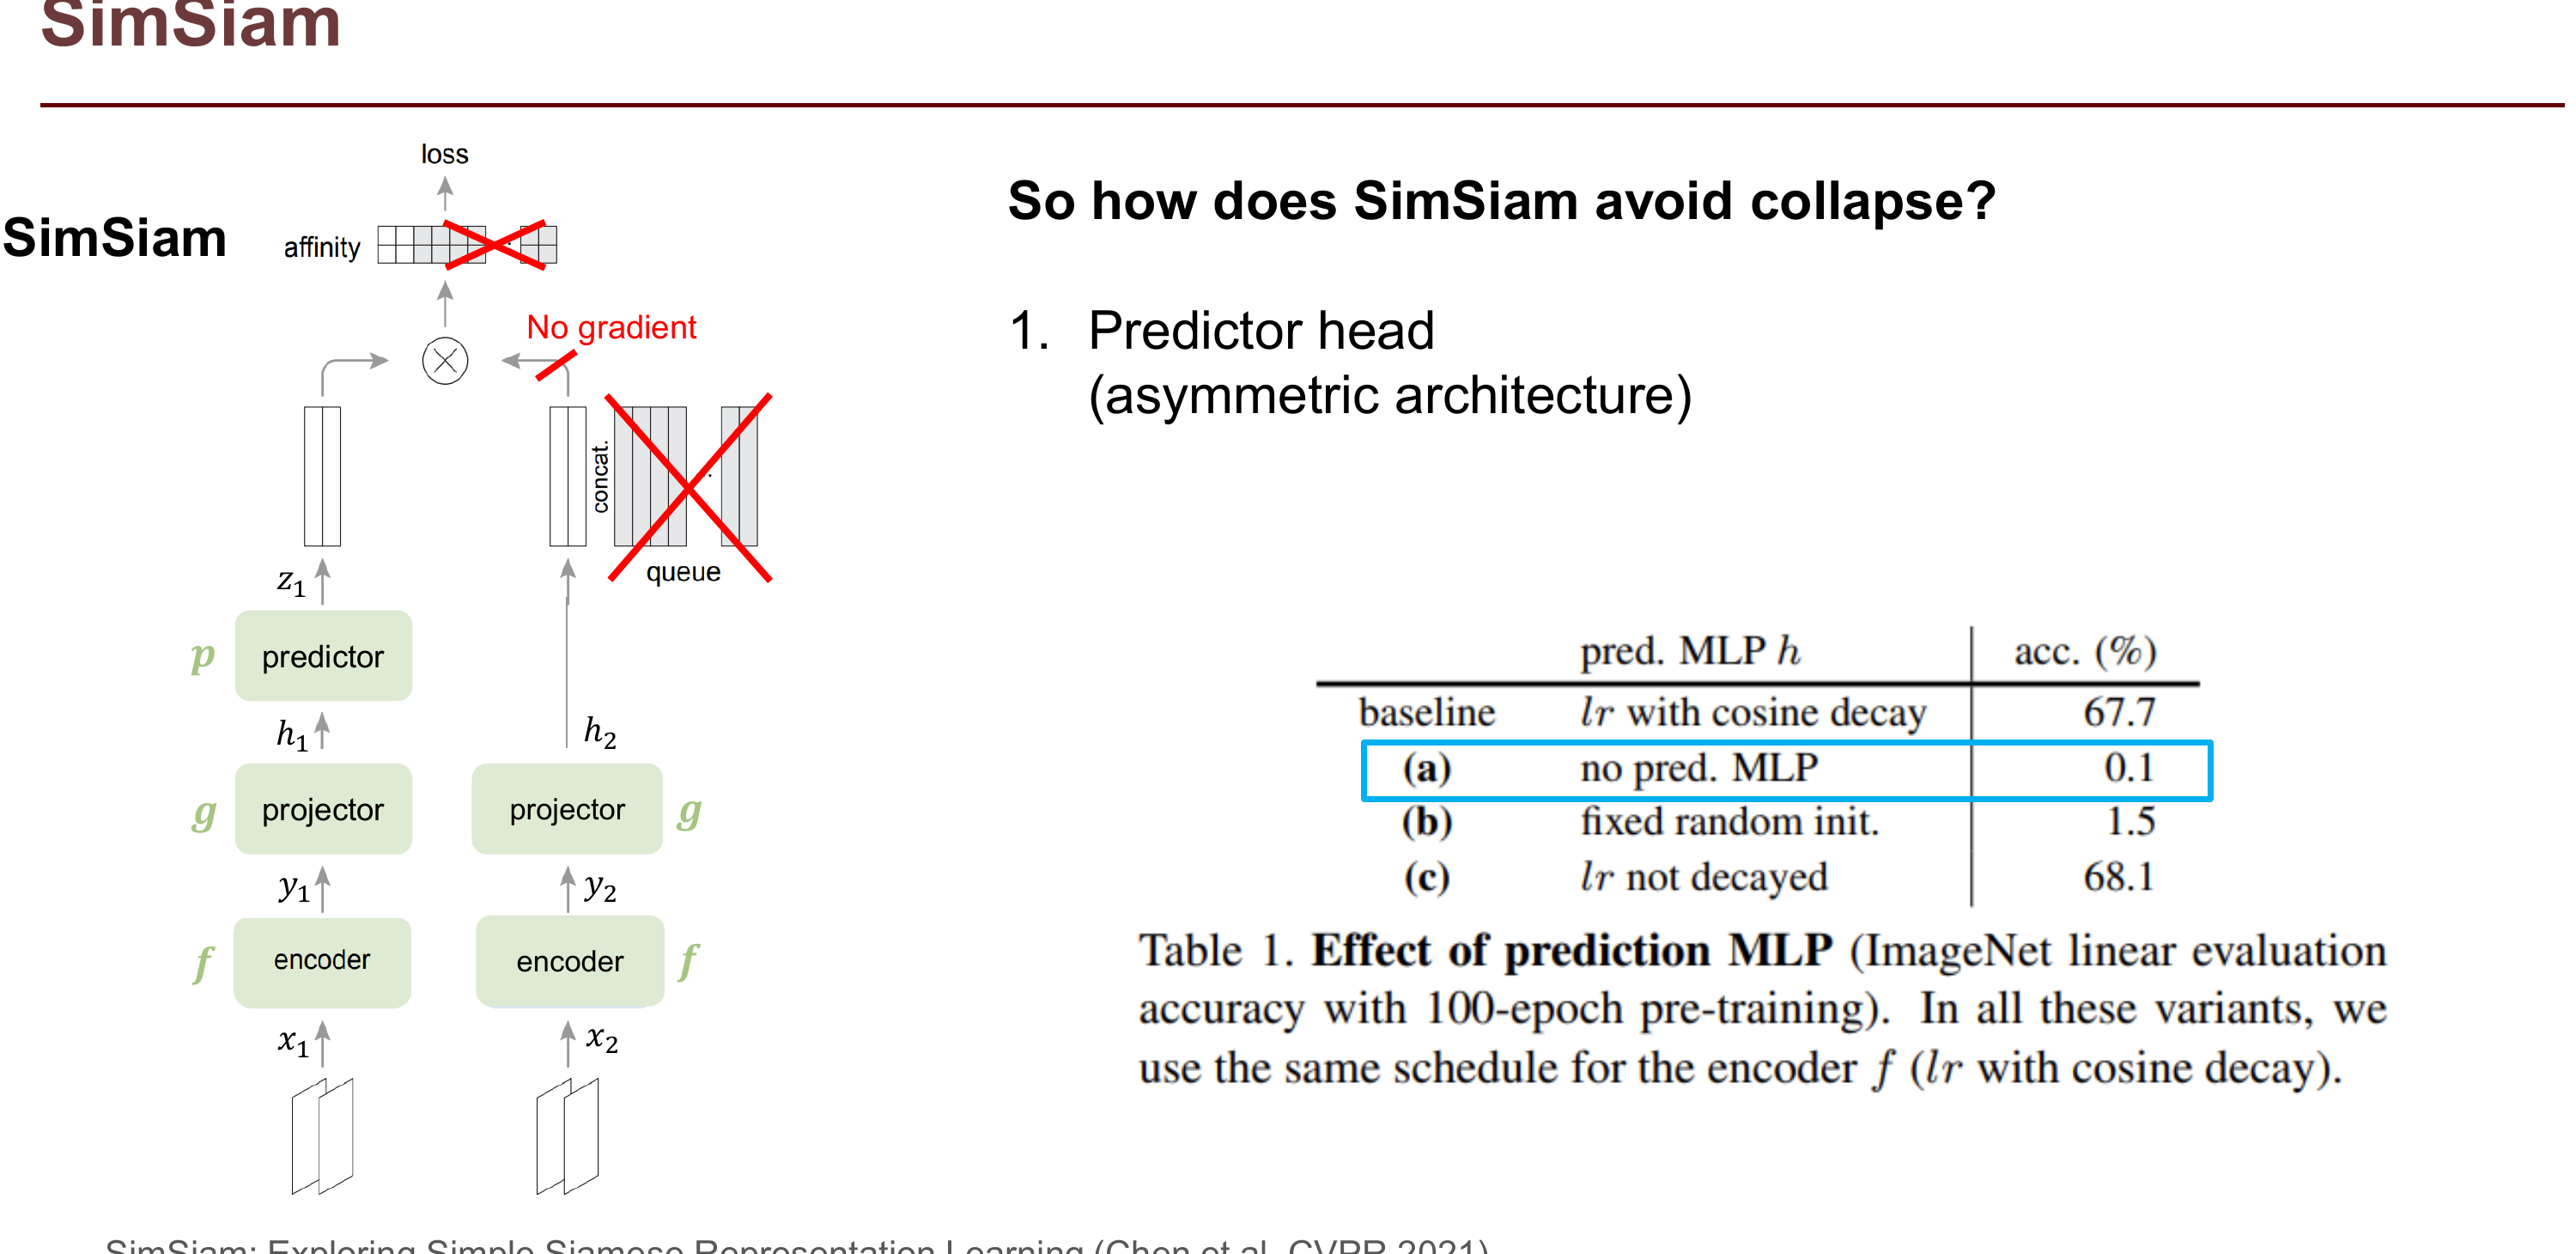
\includegraphics[width=0.90\textwidth]{Pictures/ssl_simsiam_architecture.png}
    \caption{The SimSiam architecture (from course slides~\cite{galasso2025ssl, chen2021exploring}). SimSiam operates without negative pairs and without momentum encoders, relying solely on an asymmetric predictor head and a stop-gradient operator to prevent collapse.}\label{fig:ssl_simsiam}
\end{figure}

SimSiam discards \textbf{both negative pairs and the momentum encoder}. Both branches share the exact same encoder and projector parameters $\theta$. The only asymmetric element is a predictor head $h(\cdot)$ on one branch and a \textbf{stop-gradient} ($\text{sg}$) on the other:
\begin{equation}
    \mathcal{D}(p_1, \text{sg}(z_2)) = - \frac{p_1^\top z_2}{\|p_1\|_2 \|z_2\|_2}
\end{equation}
The symmetric loss function is:
\begin{equation}
    \mathcal{L}_{\text{SimSiam}} = \frac{1}{2} \mathcal{D}(p_1, \text{stopgrad}(z_2)) + \frac{1}{2} \mathcal{D}(p_2, \text{stopgrad}(z_1))
\end{equation}

\subsubsection{Theoretical Insight: Stop-Gradient as Implicit EM Optimization}
Why does SimSiam not collapse? Chen and He hypothesized that the stop-gradient operator transforms the optimization into an implicit \textbf{Expectation-Maximization (EM-like) alternating optimization}:
\begin{equation}
    \min_{\theta} \mathbb{E}_x \left[ \min_{\eta} \mathcal{L}(\theta, \eta; x) \right]
\end{equation}
where $\eta$ represents an underlying cluster assignment or latent target representation. The inner subproblem evaluates the expectation with fixed $\theta$, while the outer subproblem updates parameters $\theta$. Removing the stop-gradient causes immediate representation collapse ($f(x) = \text{const}$).

\subsection{\texorpdfstring{DINO:\@ Self-Distillation with No Labels}{DINO (Self-Distillation with No Labels)}}

Caron et al.~\cite{caron2021emerging} formulated \textbf{DINO (Self-Distillation with No Labels)}, adapting self-supervised learning to Vision Transformers (ViT) via knowledge distillation principles, as shown in Figure~\ref{fig:ssl_dino_distillation}:

\begin{figure}[htbp]
    \centering
    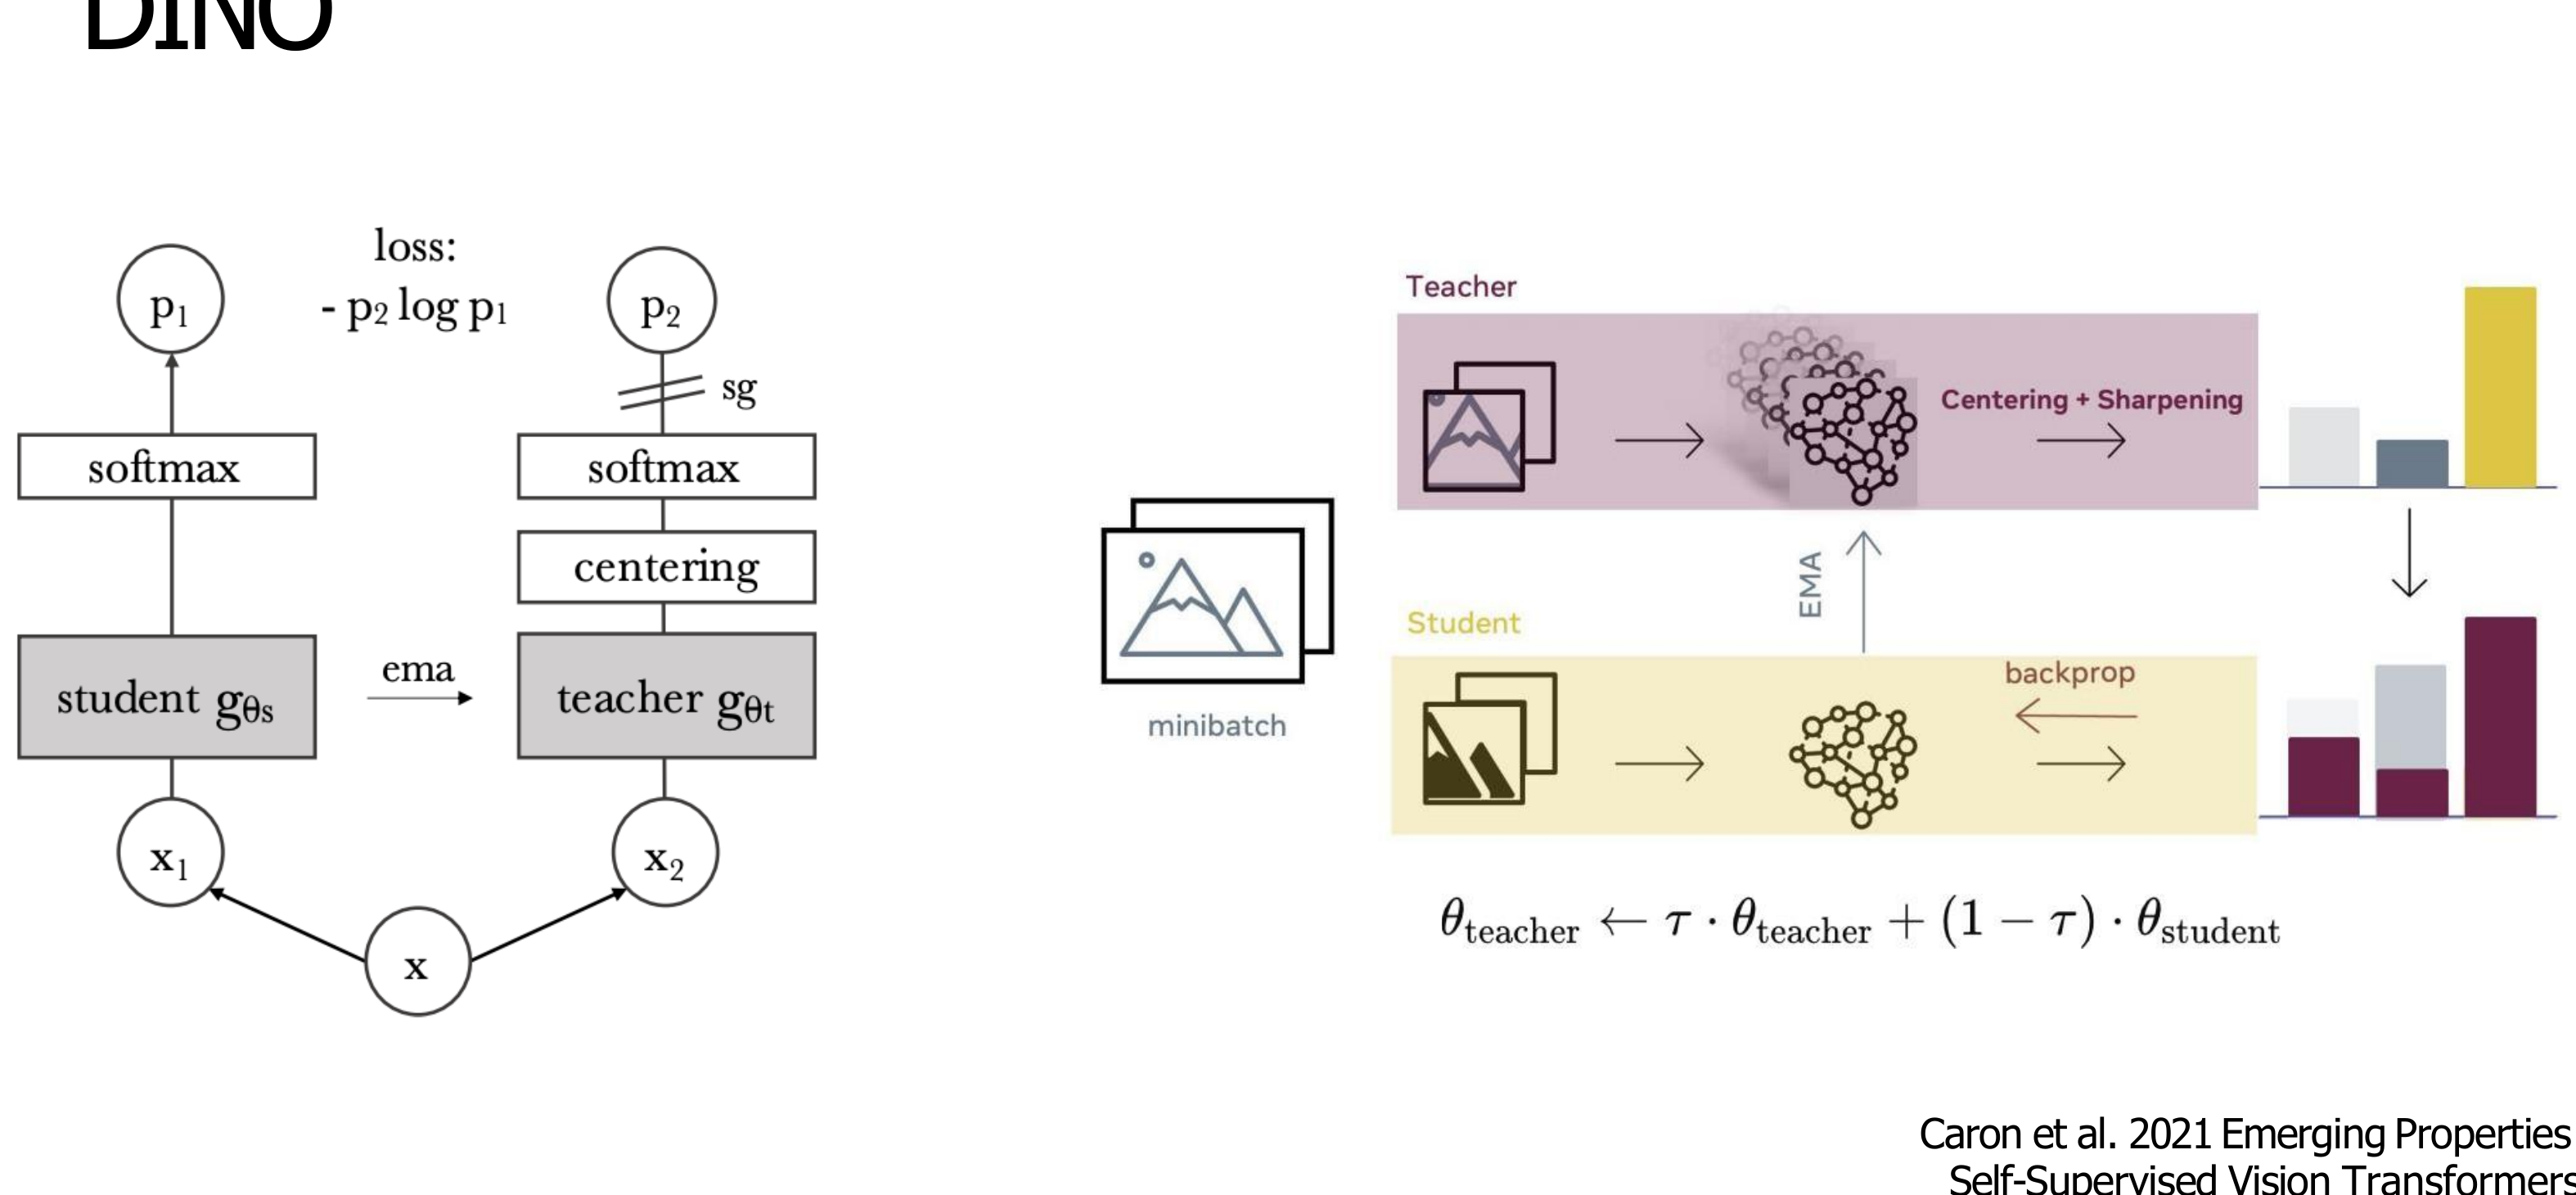
\includegraphics[width=0.92\textwidth]{Pictures/ssl_dino_distillation_architecture.png}
    \caption{DINO self-distillation architecture (from course slides~\cite{galasso2025ssl, caron2021emerging}). A student ViT learns to match the output distribution of an EMA teacher ViT. Representation collapse is avoided through centering and temperature sharpening.}\label{fig:ssl_dino_distillation}
\end{figure}

A student network $g_{\theta_s}$ and a teacher network $g_{\theta_t}$ (parameterized via EMA of the student) output probability distributions over $K$ dimensions via Softmax:
\begin{align}
    P_{s,k}(x) &= \frac{\exp(g_{\theta_s, k}(x) / \tau_s)}{\sum_{j=1}^K \exp(g_{\theta_s, j}(x) / \tau_s)} \\
    P_{t,k}(x) &= \frac{\exp((g_{\theta_t, k}(x) - c_k) / \tau_t)}{\sum_{j=1}^K \exp((g_{\theta_t, j}(x) - c_j) / \tau_t)}
\end{align}
The student minimizes cross-entropy with the teacher's predictions:
\begin{equation}
    \mathcal{L}_{\text{DINO}} = - \sum_{k=1}^K P_{t,k}(x) \log P_{s,k}(x)
\end{equation}

\subsubsection{Avoiding Collapse: Centering and Sharpening}
Without negative pairs, distillation models risk two distinct failure modes:
\begin{enumerate}[leftmargin=*]
    \item \textbf{Uniform Collapse:} All outputs degenerate into a uniform distribution $P_k(x) = 1/K$.
    \item \textbf{One-Hot Collapse:} A single dimension dominates, outputting $1$ for all inputs and $0$ elsewhere.
\end{enumerate}

DINO eliminates both failure modes through dual complementary mechanisms:
\begin{itemize}[leftmargin=*]
    \item \textbf{Centering ($c$):} A bias vector $c$ tracks the running empirical mean of teacher outputs: $c \leftarrow m c + (1 - m) \frac{1}{B} \sum_{i=1}^B g_{\theta_t}(x_i)$. Subtracting $c$ prevents any single output dimension from consistently dominating, \textbf{preventing one-hot collapse}.
    \item \textbf{Sharpening ($\tau_t < \tau_s$):} Setting a low teacher temperature $\tau_t$ (e.g., $0.04$ vs $\tau_s = 0.1$) sharpens probabilities into confident distributions, \textbf{preventing uniform collapse}.
\end{itemize}

\subsubsection{Emergence of Unsupervised Semantic Segmentation}
A remarkable breakthrough of DINO is the emergence of scene segmentation: without any human labels, the self-attention maps of the final $[CLS]$ token in a DINO-trained ViT naturally attend to the boundaries of semantic foreground objects, as shown in Figure~\ref{fig:ssl_dino_attention}.

\begin{figure}[htbp]
    \centering
    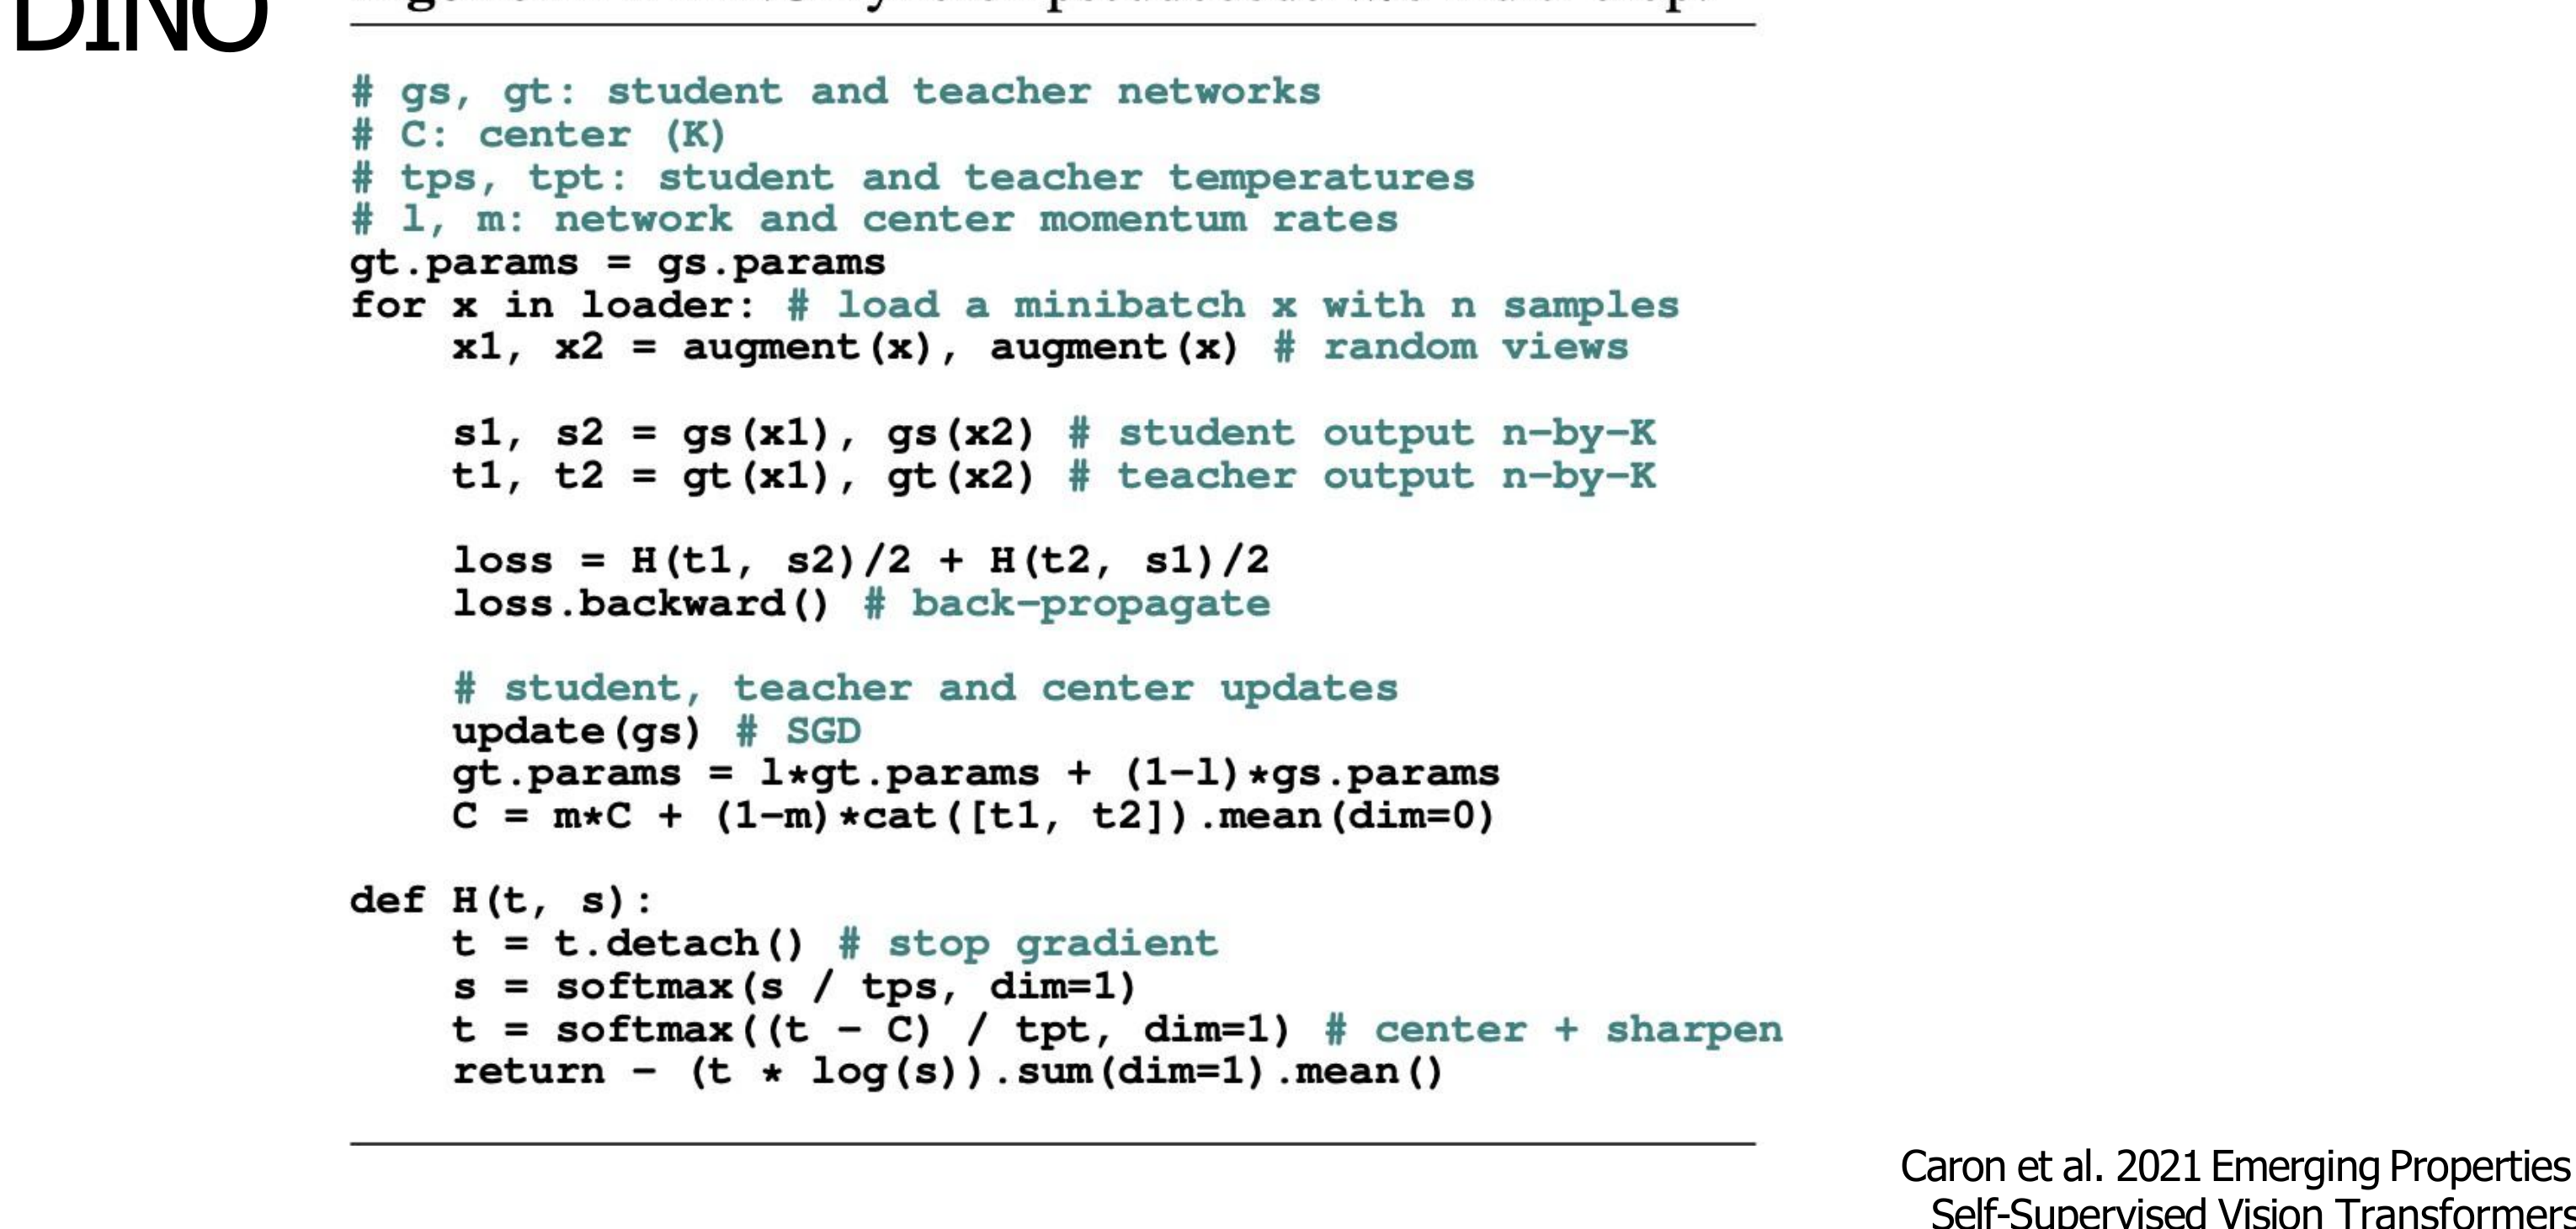
\includegraphics[width=0.90\textwidth]{Pictures/ssl_dino_attention_segmentation.png}
    \caption{Emergent unsupervised semantic segmentation in DINO (from course slides~\cite{galasso2025ssl, caron2021emerging}). The multi-head self-attention maps of a Vision Transformer trained with DINO automatically delineate semantic objects and boundaries without any segmentation labels.}\label{fig:ssl_dino_attention}
\end{figure}

Oquab et al.~\cite{oquab2023dinov2} extended this in \textbf{DINOv2}, combining image-level DINO distillation with patch-level masked modeling (iBOT) across hundreds of millions of curated images. DINOv2 generates universal, frozen visual features that achieve state-of-the-art results in monocular depth estimation, dense segmentation, and image retrieval without fine-tuning.

---

\section{Chapter Summary and Conceptual Graph}

\subsection{Comparative Summary of SSL Paradigms}

Table~\ref{tab:ssl_paradigms} summarizes the core algorithmic families analyzed in this chapter:

\begin{table}[htbp]
\centering
\small
\setlength{\tabcolsep}{3.5pt}
\begin{tabular}{p{0.16\textwidth} p{0.17\textwidth} p{0.11\textwidth} p{0.24\textwidth} p{0.24\textwidth}}
\toprule
\textbf{Paradigm} & \textbf{Key Methods} & \textbf{Negatives?} & \textbf{Anti-Collapse Mechanism} & \textbf{Primary Downstream Strength} \\
\midrule
\textbf{Heuristic Pretext} & Rotation, Jigsaw, Inpainting, Color & No & Transformation task constraints & Historical proof-of-concept; modest linear probing \\
\addlinespace
\textbf{Masked Modeling} & MAE, Context Encoders & No & High masking ratio ($75\%$) + Pixel reconstruction & Outstanding fine-tuning; state-of-the-art visual prior \\
\addlinespace
\textbf{Contrastive Learning} & SimCLR, MoCo (v1, v2) & Yes & InfoNCE negative repulsion on hypersphere & Exceptional linear probing; invariant global features \\
\addlinespace
\textbf{Non-Contrastive Siamese} & BYOL, SimSiam & No & Predictor head + Stop-gradient / EMA & High efficiency; robust to batch size constraints \\
\addlinespace
\textbf{Self-Distillation} & DINO, DINOv2 & No & Centering (mean drift) + Sharpening ($\tau_t < \tau_s$) & Unsupervised semantic discovery; dense correspondence \\
\bottomrule
\end{tabular}
\caption{Systematic comparison across modern Self-Supervised Learning paradigms.}\label{tab:ssl_paradigms}
\end{table}

\newpage
\subsection{Logical Roadmap of Representation Learning}

Figure~\ref{fig:ssl_conceptual_graph} maps the conceptual progression from supervised limitations to modern self-supervised foundation models:

\begin{figure}[htbp]
\centering
\begin{tikzpicture}[
    node distance=1.1cm and 1.5cm,
    every node/.style={font=\sffamily\small},
    conceptnode/.style={
        rectangle, 
        rounded corners=6pt, 
        draw=ocre, 
        fill=ocre!8, 
        line width=1.2pt, 
        text width=8.5cm, 
        align=center, 
        inner sep=7pt
    },
    arrowline/.style={
        -{Stealth[length=6pt, width=4pt]}, 
        draw=ocre, 
        line width=1.3pt
    }
]

\node[conceptnode] (node1) {\textbf{Supervised Learning Bottleneck}\\Annotation expense; supervision collapse to task-specific manifolds};
\node[conceptnode, below=of node1] (node2) {\textbf{Heuristic Pretext Tasks}\\Predicting rotations, patch positions, jigsaw, and inpainting};
\node[conceptnode, below=of node2] (node3) {\textbf{Generative Masked Modeling (MAE)}\\Extreme $75\%$ ViT masking, asymmetric encoder-decoder, MSE loss};
\node[conceptnode, below=of node3] (node4) {\textbf{Contrastive Learning (InfoNCE \& SimCLR)}\\Instance discrimination; NT-Xent loss; non-linear projection head};
\node[conceptnode, below=of node4] (node5) {\textbf{Decoupled Contrastive Learning (MoCo)}\\FIFO memory queue of keys; momentum encoder for temporal consistency};
\node[conceptnode, below=of node5] (node6) {\textbf{Non-Contrastive Siamese Learning (BYOL \& SimSiam)}\\Elimination of negatives; architectural predictor asymmetry; stop-gradient};
\node[conceptnode, below=of node6] (node7) {\textbf{Self-Distillation with Vision Transformers (DINO)}\\Centering \& sharpening; emergence of unsupervised semantic segmentation};

\draw[arrowline] (node1) -- (node2);
\draw[arrowline] (node2) -- (node3);
\draw[arrowline] (node3) -- (node4);
\draw[arrowline] (node4) -- (node5);
\draw[arrowline] (node5) -- (node6);
\draw[arrowline] (node6) -- (node7);

\end{tikzpicture}
\caption{Conceptual roadmap of Self-Supervised Learning paradigms.}\label{fig:ssl_conceptual_graph}
\end{figure}

\begin{InsightBox}
\textbf{Connecting the Self-Supervised Paradigms:} \\
\begin{itemize}[leftmargin=*]
    \item \textbf{Supervised $\to$ Heuristic:} Replacing manual annotations with data-driven transformations eliminates human labeling but risks low-level heuristic shortcuts.
    \item \textbf{Heuristic $\to$ Masked Modeling (MAE):} Elevating inpainting to Vision Transformers with $75\%$ masking forces holistic semantic scene understanding while slashing encoder computational cost.
    \item \textbf{Heuristic $\to$ Contrastive Learning:} Replacing domain heuristics with task-agnostic instance discrimination maps semantic views to a unit hypersphere via mutual information maximization.
    \item \textbf{SimCLR $\to$ MoCo:} Decoupling dictionary size from mini-batch size via a dynamic FIFO memory queue and momentum encoder enables massive negative sets on standard hardware.
    \item \textbf{Contrastive $\to$ Non-Contrastive (BYOL/SimSiam):} Proving negative samples are unnecessary; architectural asymmetry and stop-gradient prevent representation collapse.
    \item \textbf{Non-Contrastive $\to$ Self-Distillation (DINO):} Unifying ViT distillation with centering and sharpening yields representations with emergent, unsupervised semantic segmentation capabilities.
\end{itemize}
\end{InsightBox}
